% TODO https://trello.com/
%
\chapter{Software Configuration Management}
Als Konfiguration eines Systems bezeichnet man die Festlegung seiner
Elemente mit ihren Versionen resp. Varianten:
(\href{http://www.software-kompetenz.de/?22704}
{www.software-kompetenz.de/?22704})
\begin{quote}
Eine Konfiguration ist ein Entwicklungsstand eines Produkts, in dem neben dem
Quellcode und der Dokumentation sämtliche Werkzeuge und Hilfsmittel zum
Erzeugen einer lauffähigen Version zusammengefasst sind. Das schließt auch die
Dokumentation und die Einstellungen bzw. verwendete Parameter der Werkzeuge
und Hilfsmittel ein.
\end{quote}
\newslide
Softwaresysteme sind aus vielfältigen Gründen \"Anderungen unterworfen:
Strategie- und Marketingentscheidungen, Fehlerbehebungen, Kundenforderungen,
nicht mehr unterstützte Softwareversionen von Drittherstellern etc.

\newslide
Änderungen betreffen meist unterschiedliche, von einander abhängige Elemente
\begin{itemize}
\item Anforderungskatalog, Spezifikation, Pflichtenheft
\item Designspezifikation
\item Testplan, Testreport, Testspezifikation
\item Projektplan
\item Quell-Kode
\item Makefiles
\item Produkte von Drittherstellern (Compiler, Libraries, Datenbank \ldots)
\item Benutzerhandbuch, Administrationsanweisungen
\item Ausbildungsunterlagen, Marketingbrochuren,
\item \ldots
\end{itemize}
Unkontrolliert durchgeführte Änderungen an einem oder mehreren Elementen
können unversehends zu Funktionsstörungen oder anderen Inkonsistenzen
führen.

Deshalb: Um die Integrität und Rückverfolgbarkeit eines Softwaresystems zu
gewährleisten, muss ein
systematischer Änderungsprozess betrieben werden:
\begin{quote}
Configuration Management ... is a management process for establishing and
maintaining consistency of a product's performance, its functional and
physical attributes, with its requirements, design and operational
information, throughout its life. (ANSI/EIA)
\end{quote}
\newpage
\section{Gliederung (IEEE/SWEBOK)}
\begin{figure}[H]
\centering
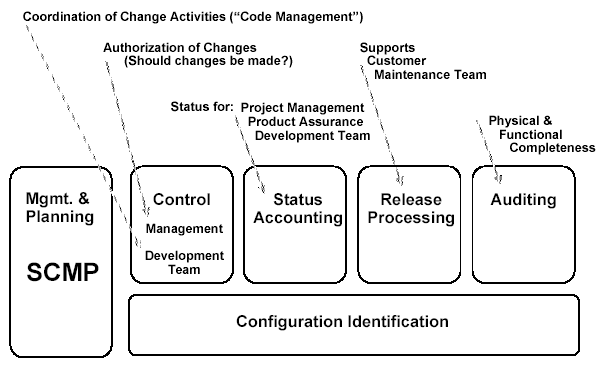
\includegraphics[width=0.75\linewidth]{config-management/scm-activities}
\caption{Software Configuration Management (Source: SWEBOK)}
\end{figure}
\begin{itemize}
\item \underline{SCMP}
   (Management des Software-Konfigurationsprozesses):
  \begin{itemize}
  \item Organisatorischer Kontext: Einbindung in die betriebliche
  Organisation, Bezeichnung der Schnittstellen und Verantwortlichkeiten,
\item Randbedingungen und Wegleitung: Berücksichtigung juristischer,
  ökonomischer, unternehmenspolitischer Faktoren, Anwendung von
  ``Best-Practices''
\item Planung: Festlegung und Anpassung der Verfahren und Werkzeuge zur
  Identifikation der Software-Elemente, Steuerung und Überwachung des
  Prozesses, Release-Management und Auslieferung, unter Berücksichtigung des
  Projektumfanges
  \end{itemize}
\item \underline{Configuration Identification} (Identifikation):
 Festlegung und Beschreibung der Bezugskonfiguration (Baseline),
  Markierung der Elemente, Aufnahme in die Konfiguration,
  Zulassungsverfahren (approval), Bezeichnung der Software-Bibliotheken
\item \underline{Control} (Steuerung):
  formelle Organisation und Behandlung von Änderungen,
  Strukturierung der Anfragen (Requests), Abschätzung der Auswirkungen,
  Durchführung und Freigabe, Umgang mit Abweichungen (Verzichtserklärungen)
\item \underline{Status Accounting} (Buchführung): Aufzeichnung der Aktivitäten mit
  Terminangaben und
  kommentierenden Erläuterungen, Ablageverfahren, Berichterstattung
\item \underline{Auditing} (Überwachung): Einhaltung der Vorgaben,
  Durchführung von Audits
%Evaluation von Verbesserungen
\item \underline{Release Processing} (Release-Managemement und Auslieferung):
  Festlegung,
  Erstellung und
  Beschreibung der auszuliefernden Konfiguration (Release Notes: neue
  Funktionalität, bekannte
  Einschränkungen und Probleme, Plattform-Anforderungen), Mitteilung an Kunden
\end{itemize}
%\newpage
%----------------------------------------------------------------------
\section{Versionen, Revisionen und Ausgaben}
Ein File (Dokument) kann verschiedene Versionen haben:
\begin{figure}[H]
\begin{center}
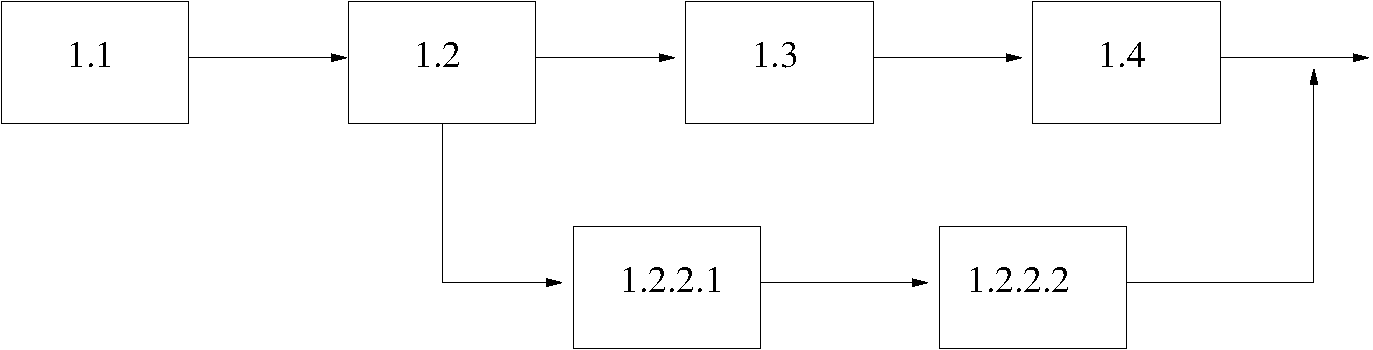
\includegraphics[width=0.8\linewidth]{config-management/xfig/file-revisions}
\end{center}
\caption{Die Versionen einer Datei}
\end{figure}
Sie werden \underline{Revisionen} (engl. Revisions) genannt.

\ifslides
\else
Ebenso kann ein Softwareprodukt mehrere Versionen haben. Man
nennt sie \underline{Ausgaben} (engl. Releases). Ihre Sourcefiles
haben jedoch unterschiedliche Versionen:

\fi
\begin{figure}[H]
\begin{center}
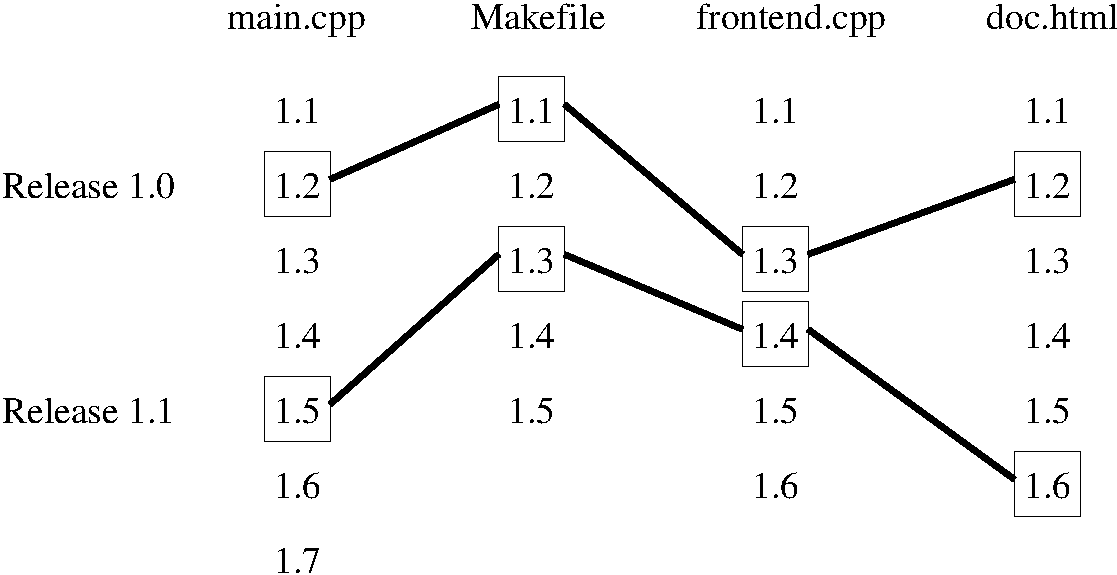
\includegraphics[width=0.9\linewidth]{config-management/xfig/releases}
\end{center}
\caption{Die Versionen eines Produktes}
\end{figure}
\newslide

Die Entwicklung erfolgt normalerweise entlang des Hauptastes
(Trunk oder Master). In mehreren Zyklen werden Dateien modifiziert,
hinzugefügt, gelöscht und umbenennt.

Bevor ein neuer Release gebildet wird, empfiehlt es sich
eine Verzweigung (Branch) zu erstellen. Dieser Moment wird auch als
``Code'' resp. ``Feature freeze'' bezeichnet, da innerhalb dieser Verzweigung
keine funktionalen Erweiterungen sondern nur noch diejenigen
Änderungen durchgeführt werden, die für die Integrations- und
Systemtests nötig sind. Nach Abschluss dieser Phase sollten die
Änderungen wieder mit dem Hauptast zusammengeführt werden.
\begin{figure}[H]
\begin{center}
  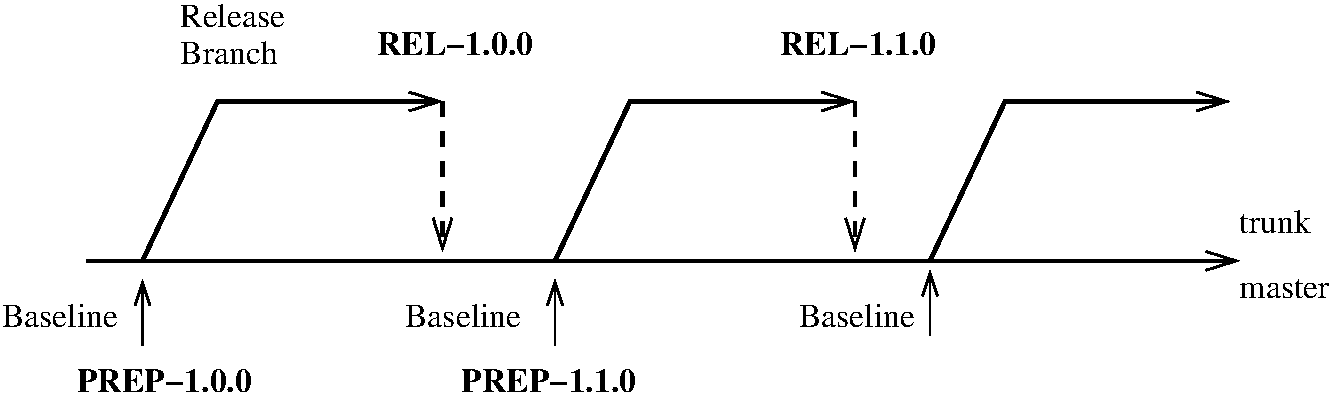
\includegraphics[width=0.9\linewidth]{config-management/xfig/release-branch}
\end{center}
\caption{Release-Bildung mit Branches und Merges}
\end{figure}
Die nicht mit dem Release beschäftigten Entwickler können während der
Release-Bildung auf dem Trunk weiterarbeiten.

\newslide
Für die Release-Bezeichnung empfiehlt es sich, ein einfaches und
nachvollziehbares Schema
anzuwenden. Z. B: {\bfseries major.minor.patch}

\begin{tabular}{ll}
Major: & umfangreiche Änderungen oder Erweiterungen\\
Minor: & zusätzliche Funktionalitäten\\
Patch: & Fehlerbehebungen oder geringfügige Verbesserungen\\
\end{tabular}

% Siehe http://apr.apache.org/versioning.html
%---------------------------------------------------------------
\newpage
%\subsection*{Konfigurationsmanagement}
\section{Change Management}
\begin{figure}[H]
\ifslides
\begin{center}
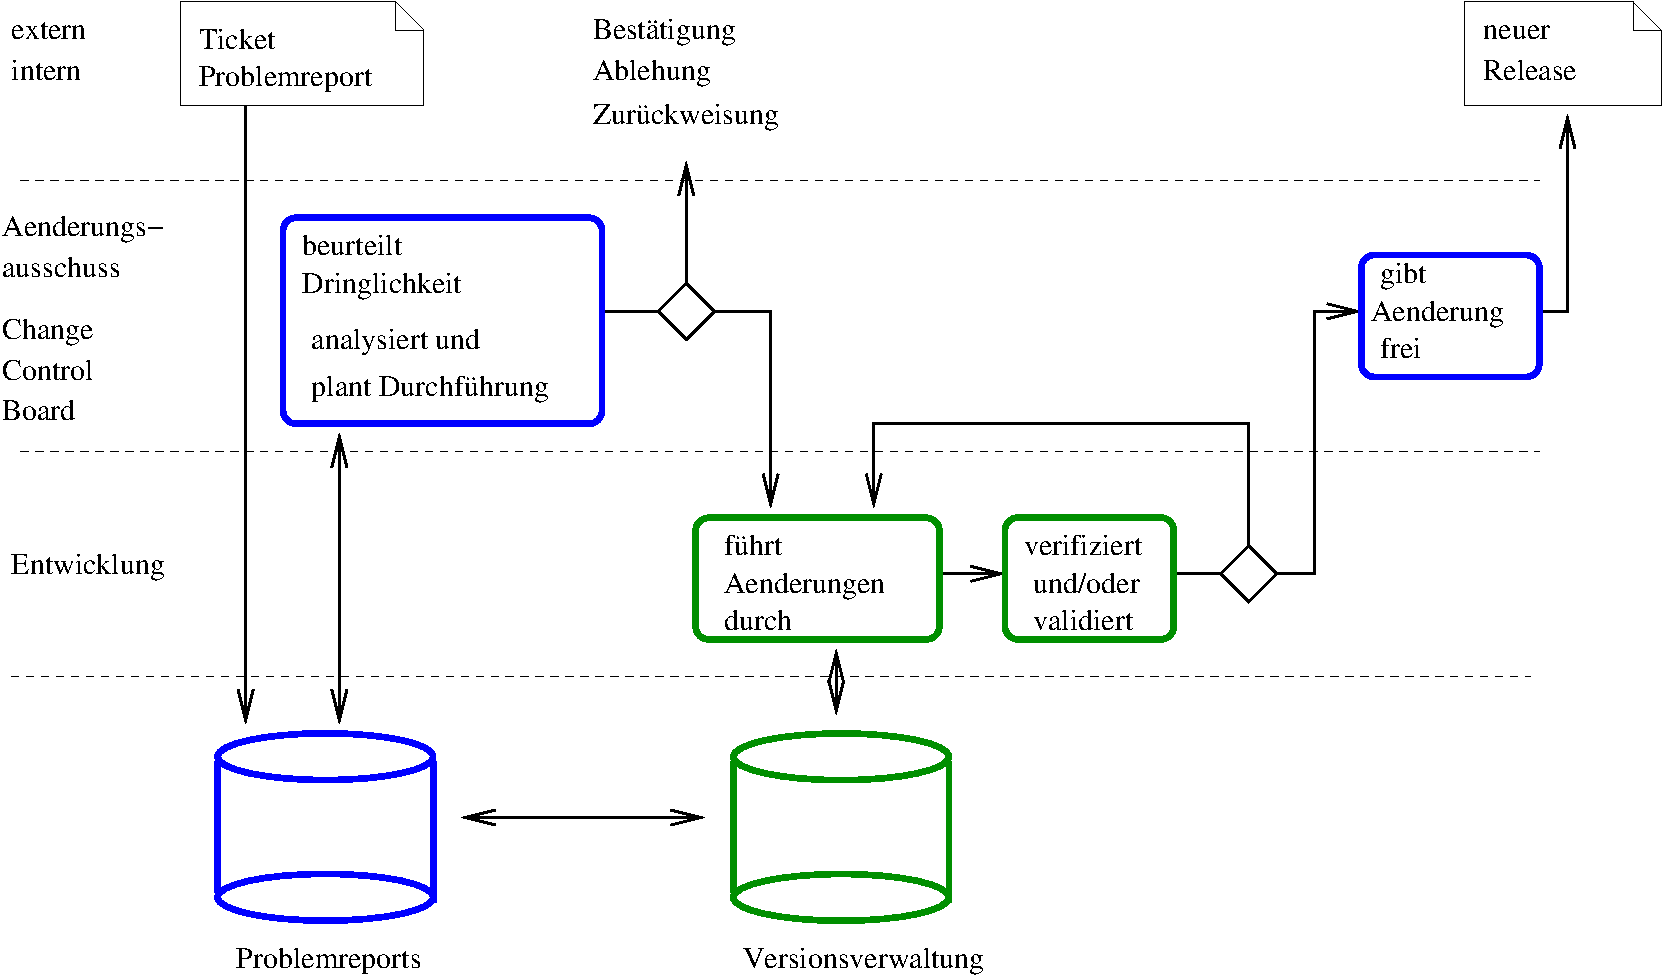
\includegraphics[width=0.65\linewidth]{config-management/xfig/changemgmt}\\[2ex]
\end{center}\else
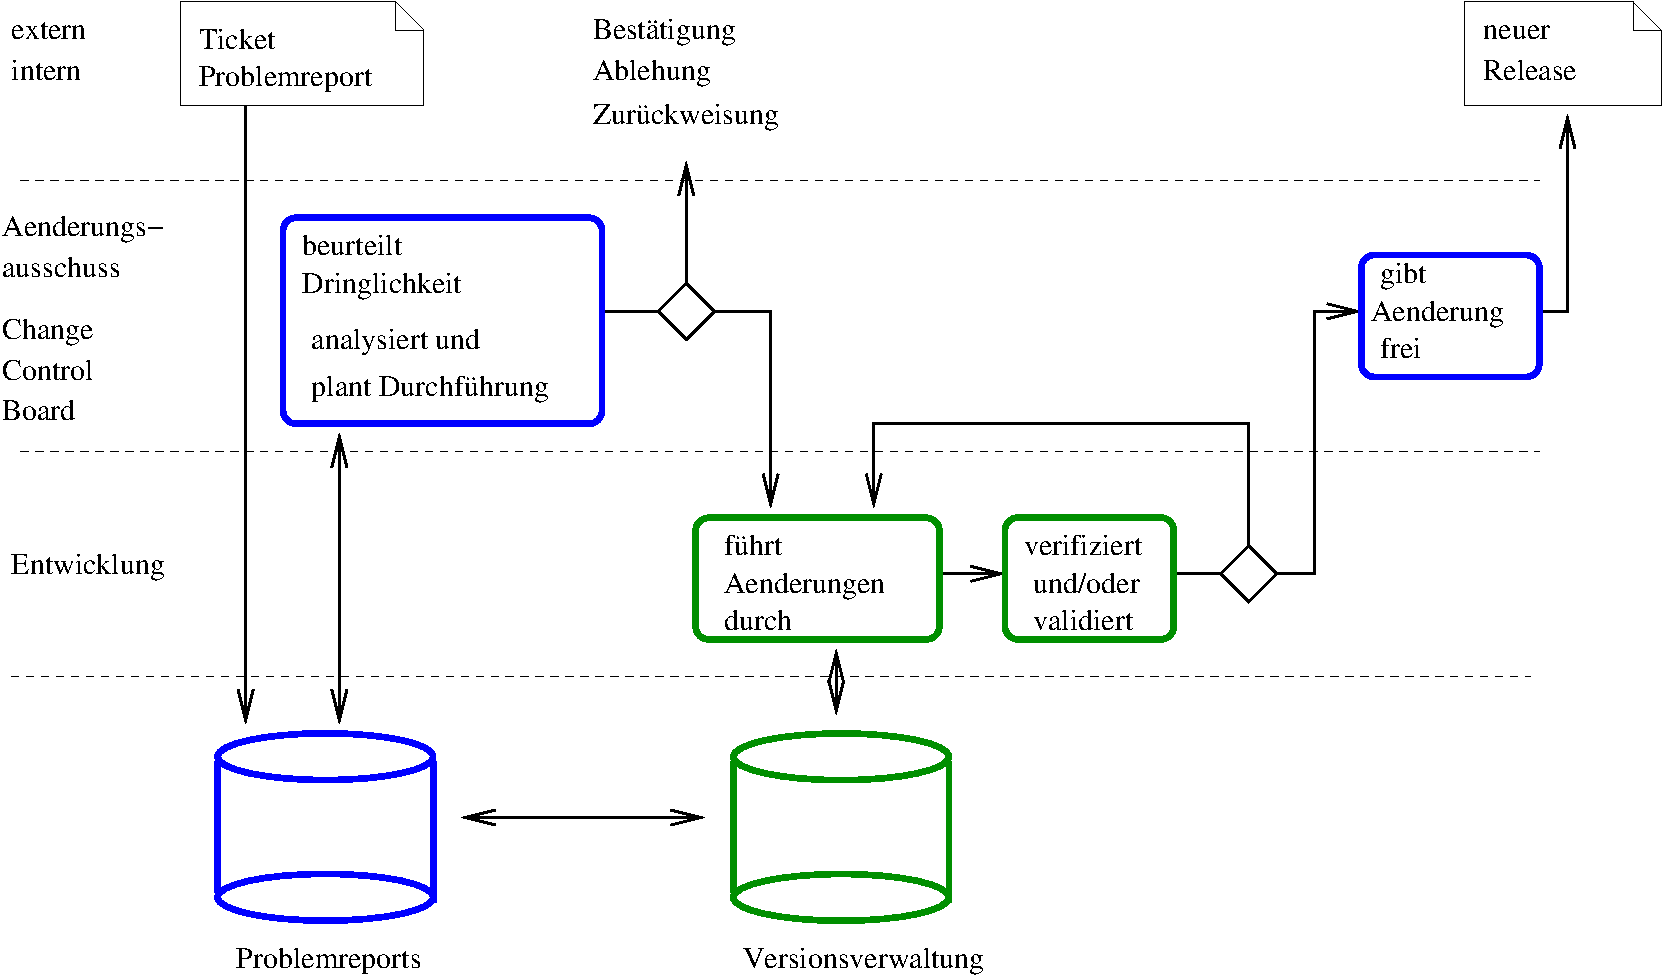
\includegraphics[width=\linewidth]{config-management/xfig/changemgmt}
\caption{Der Änderungsprozess}
\fi
\end{figure}
\begin{minipage}[t]{0.48\linewidth}
\subsection*{Bug and Issue Tracking} %Problembehandlung
\begin{itemize}
\item Erfassung und Verwaltung aller eingehender Fehlermeldungen
  und \"Anderungsanträgen
\item Entscheidung über die Bearbeitung der Meldungen unter Berücksichtigung
 der technischen und zeitlichen Auswirkungen
\item Abschluss der \"Anderung und Information der Betroffenen
\end{itemize}
\end{minipage}
\hfill
\begin{minipage}[t]{0.48\linewidth}
\subsection{Version Control}
\begin{itemize}
\item Eindeutige Kennzeichnung der Software-Elemente
\item Einfrieren von Zwischenergebnissen
\item Sicherstellen dass auf vorangegangene Versionen
  zurückgegriffen werden kann
\end{itemize}
\end{minipage}
\newslide
\section{Software and further Informations}
\begin{itemize}
\item Software Engineering Body of Knowledge (Kap. 7 SCM):
  \href{http://www.swebok.org}{www.swebok.org}
\item Eine nützliche  Linksammlung: \href{http://www.cmcrossroads.com/yp}
                                          {www.cmcrossroads.com/yp/}
\end{itemize}
%---------------------------------------------------------------
\newslide
% CRISP: Complete Repeatable Informative Schedulable Portable
% (Pragmatic Project Automation)
%
\section{The Software Build Process}
Die Aufgabe des Erstellungs- (od. Build)-Prozesses in der
SW-Entwicklung ist es, die
benötigten Produkte (Artefakte) in einer konsistenten,
reproduzierbaren und soweit wie möglich
automatisierten Weise zu erstellen.

In der Regel umfasst
dieser Prozess die folgenden Schritte:
\begin{itemize}
\item Erstellen von Resource- und Quellkodedateien %Identifikation der Elemente
\item Kompilieren und Linken
\item Testen
\item Generierung der Dokumentation
\item Verpacken
\item Installation
\item Deployment
\end{itemize}
Damit der Erstellungsprozess automatisiert und reproduzierbar
durchgeführt werden kann,
benötigt man eine Beschreibung der auszuführenden Programme
(Kompiler, Linker\ldots) inklusive der jeweiligen Aufrufparameter und
ihrer Abhängigkeiten. Dazu werden oft auf Basis von Dateiendungen (.java,
.class) bestimmte Ausführungsregeln definiert.
Von entscheidender Bedeutung und meist besonders heikel
ist auch das korrekte Einbinden der
verwendeten Bibliotheksdateien.

Der Erstellungsprozess soll sich am Prinzip \structure{CRISP} orientieren:

 {\bfseries C}omplete {\bfseries R}epeatable {\bfseries I}nformative {\bfseries S}chedulable {\bfseries P}ortable

Verbreitete Werkzeuge zur Unterstützung des Erstellungsprozesses sind:
\begin{itemize}
\item make, CMake und Automake/Autotools (Unix, Windows/Cygwin)
\item Apache Ant
\item Apache Maven
\item Gradle
\end{itemize}
%
\subsection{Ant}
Ant ist ein Java-basierendes Open-Source-Werkzeug zur Steuerung von
  Generierungsabläufen wie
  zum Beispiel das Kompilieren von Java-Klassen und das Verpacken
zu Archivdateien. Gemäss James Duncan
  Davidson, der dieses mittlerweile zum De-Facto-Standard gewordene Tool 1998
  entwickelt hat, ist ANT die Abkürzung von ``Another Neat Tool''.

Um Ant zu verwenden, muss eine sogenannte Build-Datei in XML-Format erstellt
werden. Diese Datei hat folgende Eigenschaften:
\begin{itemize}
\item Jede Ant-Build-Datei
   enthält genau ein {\bfseries Projekt}-Element mit einem Default-Target.
\item Jedes Ant-Projekt besteht aus einem oder mehreren {\bfseries Targets}, in
  welchen {\bfseries Tasks} ausgeführt werden.
\end{itemize}
\newslide
Beispiel:
\begin{lstlisting}[language=xml,morekeywords={project,target,javac,mkdir}]
<project name="SimpleProject" default="compile">

  <target name="init">
    <mkdir dir="build"/>
  </target>

  <target name="compile" depends="init">
    <javac srcdir="src"
        destdir="build"/>
  </target>
</project>
\end{lstlisting}
\ifslides
\else
Die obige Datei sorgt dafür, dass
\begin{enumerate}
\item das Verzeichnis \verb+build+ erstellt wird, falls es nicht
  bereits existiert (ACHTUNG: Ant besteht auf dem Verzeichnistrennzeichen
  \verb+/+ und nimmt system-spezifische Anpassungen automatisch vor),
\item alle Java-Dateien, die sich im Verzeichnis src und darunter befinden,
   werden kompiliert und die daraus entstehenden Class-Dateien ins Verzeichnis
  \verb+build+  geschrieben.
\end{enumerate}
\fi
\newslide
Ein Ant-Prozess kann wie folgt angestossen werden:

\begin{tabularx}{\linewidth}{l|X}
Aufruf   & Bedeutung \\
\hline
ant  &  führt das Default-Target, der im aktuellen
  Verzeichnis liegenden Datei build.xml, aus.\\
%\hline
ant -f otherbuild.xml & verwendet otherbuild.xml als
  Build-Datei. \\
%\hline
ant compile & führt das Target {\bfseries compile}
  aus.\\
%\hline
ant -projecthelp & zeigt die verfügbaren Targets an.\\
%\hline
ant -version & zeigt die aktuelle Ant-Version an.\\
%\hline
ant -emacs & erzeugt von Emacs auswertbare Log-Meldungen.\\
\end{tabularx}

Standardmässig bringt Ant über 80 Tasks mit, die einen breiten
Anwendungsbereich abdecken und die auch durch eigene Tasks erweitert werden
können. Es gibt über 100 Erweiterungsprojekte und Tools zu Ant.
%
\newslide
\subsubsection{Konstanten}
Um allenfalls notwendige Anpassungen zu vereinfachen, sollten in der
Build-Datei Konstanten als sogenannte Properties vereinbart werden:
\begin{lstlisting}[language=xml, morekeywords={property,target,javac}]
<property name="build.dir" value="build"/>
<target name="compile">
  <javac srcdir="src"
        destdir="${build.dir}"/>
</target>
\end{lstlisting}
%$
Oft sind diese auch in einer separaten Datei definiert:
\begin{lstlisting}[language=xml,morekeywords={property}]
<property file="project.properties"/>
\end{lstlisting}
In der Datei project.properties sind die Werte zeilenweise aufgeführt:
\begin{verbatim}
build.dir=build
\end{verbatim}
%
\newslide
\subsubsection{Erstellung einer Archiv-Datei}
Eine Archiv-Datei kann mit dem Task jar erstellt werden:
\begin{lstlisting}[language=xml,morekeywords={target,jar,mkdir}]
<target name="dist" depends="compile"
   description="generate the distribution" >
   <mkdir dir="dist" />
   <jar destfile="dist/project.jar"
        basedir="${build.dir}"/>
</target>
\end{lstlisting}
%$
Das Attribut destfile legt den Filenamen fest und mit basedir wird
das Verzeichnis bezeichnet, dessen Dateien in die Archiv-Datei
aufgenommen werden.

\newslide
Um eine Archiv-Datei ausführbar zu machen, muss eine Manifest-Datei
mit folgendem Inhalt hinzugefügt werden:
\begin{verbatim}
  Main-Class: classname
\end{verbatim}
wobei \verb+classname+ die Klasse bezeichnet, welche die Main-Methode
enthält. In der Ant-Build-Datei kann dies mit dem Element manifest
vereinbart werden:
\begin{lstlisting}[language=xml,morekeywords={jar,manifest,attribute}]
   <jar destfile="dist/project.jar"
        basedir="${build.dir}">
      <manifest>
	<attribute name="Main-Class"
		   value="example.Main"/>
      </manifest>
   </jar>
\end{lstlisting}
%$
\newslide
\subsubsection{Filesets}
Mit Filesets können Dateien gruppiert werden:
\begin{lstlisting}[language=xml,morekeywords={fileset,include,exclude}]
<fileset dir="src">
  <include name="**/*.java"/>
  <exclude name="**/*Test*"/>
</fileset>
\end{lstlisting}
Hiermit wird eine Gruppe gebildet mit allen Java-Dateien, die im
src-Verzeichnis und darunter liegen und nicht den Text ''Test'' im
Namen enthalten.
%
\newslide
\subsubsection{Pfade}
Als Pfad bezeichnet man eine Sammlung von Ressourcen (Dateien), die
üblicherweise mit einem Id-Attribut eindeutig gekennzeichnet werden:
\begin{lstlisting}[language=xml,morekeywords={path,pathelement,fileset,include}]
<path id="compile.classpath">
  <fileset dir="lib">
    <include name="**/*.jar"/>
  </fileset>
</path>

<path id="run.classpath">
  <pathelement location="${build.dir}"/>
  <path refid="compile.classpath"/>
</path>
\end{lstlisting}
%$
\newslide
Damit kann beim Compilieren der Klassenpfad wie folgt gesetzt werden:
\begin{lstlisting}[language=xml,morekeywords={javac,classpath}]
<javac ...>
  <classpath refid="compile.classpath"/>
</javac>
\end{lstlisting}
und beim Ausführen:
\begin{lstlisting}[language=xml,morekeywords={java,arg,classpath}]
<java classname="test.Main">
  <arg value="-h"/>
  <classpath refid="run.classpath"/>
</java>
\end{lstlisting}
%
\newslide
\subsubsection{Exercise}
\begin{enumerate}
\item Erstellen Sie eine Ant-Build-Datei für das Projekt
Histogram\footnote{Download:
\href{http://download.semafor.ch/courses/histo.zip}
  {download.semafor.ch/courses/histo.zip}},
  welche die Java-Dateien kompiliert und die erzeugten Class-Dateien in die
  ausführbare Jar-Datei \verb+histogram-YYYYMMDD.jar+ verpackt,
  wobei YYYYMMDD das aktuelle Datum bedeutet. Verwenden Sie dazu
  den Ant-Task \verb+tstamp+. Beispiel:
\begin{lstlisting}[language=xml,morekeywords={tstamp,echo,target}]
<target name="hello">
  <tstamp/>
  <echo message="Hello, today is: ${DSTAMP}"/>
</target>
\end{lstlisting}
%$
Das Projekt Histogram benötigt die JFreeChart-Bibliotheken
jfreechart-1.0.12.jar und jcommon-1.0.15.jar
 von
\href{http://www.jfree.org/jfreechart}{www.jfree.org/jfreechart}.
Diese befinden sich im lib-Verzeichnis nach dem Entpacken.

Tipp: Sorgen Sie dafür, dass die erstellte JAR-Datei alle benötigten Klassen
enthält, indem Sie das Zipfileset-Element verwenden.
\end{enumerate}
%
\newslide
\subsubsection{Software and further Informations}
\begin{itemize}
\item Java Development with Ant (Erik Hatcher, Steve Loughan), Manning
  Publications
\item Das Apache ANT Projekt:
  \href{http://ant.apache.org}{ant.apache.org}
\item Apache Ant:
  \href{http://en.wikibooks.org/wiki/Programming:Apache_Ant}
     {en.wikibooks.org/wiki/Programming:Apache\_Ant}
\item Ant Wiki:
  \href{http://wiki.apache.org/ant/FrontPage}{wiki.apache.org/ant/FrontPage}
\item Introduction to
  Ant:\href{http://www.exubero.com/ant/antintro-s5.html}
{www.exubero.com/ant/antintro-s5.html}
\end{itemize}
%
\newslide
%
% http://pettermahlen.com/2010/05/01/code-sharing-use-maven/
%
\subsection{Maven}
Wie Ant ist auch Maven ein Open-Source-Werkzeug zur einfachen Automatisierung von
Build-Prozessen.

\ifslides
Vorteile:
\begin{itemize}
\item Reduzierter Konfigurationsaufwand:
       {\em deklarativ} statt {\em imperativ}, Convention over Configuration
\item Paket-Management mit Versionierung: Repository für Libraries
\item Einheitlicher Build-Prozess mit Standardverzeichnisstruktur
\item IDE-Unabhängigkeit: Unterstützung von Eclipse, Netbeans, Intellij
\end{itemize}
\else
Im Unterschied zu Ant basiert Maven jedoch auf einem
{\em deklarativen} anstelle eines {\em imperativen} Ansatzes:
man beschreibt {\em was} und
nicht {\em wie} man etwas tun will. Die Folge davon ist ein
wesentlich geringerer Konfigurationsaufwand.
Zusätzlich orientiert sich Maven am Prinzip ``Convention over
Configuration'': hält man sich an die von Maven vorgeschlagene
Verzeichnisstruktur, vereinfacht sich die Konfiguration entsprechend.

Eine weitere wertvolle Eigenschaft von Maven ist die Fähigkeit
die verwendeten Bibliotheken (sog. Artefakte) zu verwalten.
Maven holt sich bei Bedarf
die benötigten Archivdateien vom Internet herunter und legt sie
in ein zentrales Repository.

Von Haus aus bringt Maven bereits
einen Standard-Build-Prozess mit und etabliert damit
eine einheitliche Projektstruktur. Auch dies ein nicht zu
unterschätzender Vorteil. Ausserdem kann Maven unabhängig von einer IDE
benutzt werden, es unterstützt aber auch die
Entwicklungsumgebungen Eclipse, Netbeans und Idea.

Die erste Version von Maven, die 2002 in relativ kurzer Zeit
eingeführt wurde, wies noch einige Unzulänglichkeiten
auf. Mittlerweile ist eine in wesentlichen Teilen erneuerte und
verbesserte Version 2 (resp. 3) verfügbar. Diese Versionsproblematik
kann jedoch auf einigen Internet-Seiten noch für etwas Verwirrung
sorgen.
\fi
\newslide
%
\subsubsection{Projektmodell}
Grundlage des Erstellungsprozesses von Maven ist das Projektmodell (POM).
Es beschreibt die Metadaten, Abhängigkeiten und alle notwendigen
Angaben damit Maven den entsprechenden Build-Prozess
durchführen kann:
\begin{itemize}
\item \structure{Allgemeine Angaben}: Projektkoordinaten, Verpackungsart \ldots
\item \structure{Dependencies}: Abhängigkeiten zu externen Bibliotheken,
\item Build: spezielle Angaben zum Build-Prozess (plugins),
\item Properties: projekt-spezifische Konstanten,
\item Profile: Build-Varianten,
\item Repositories: spezielle Verzeichnisse für die verwendeten
  Bibliotheken und Plugins,
\item Reporting: Projektdokumentation
\end{itemize}
Diese Angaben werden in der XML-Datei pom.xml abgelegt. Beispiel:
\begin{lstlisting}[language=xml,
   morekeywords={modelVersion,groupId,artifactId,
   packaging,version,name,url,dependencies,dependency,scope,project}]
  <project xmlns="http://maven.apache.org/POM/4.0.0"
       xmlns:xsi="http://www.w3.org/2001/XMLSchema-instance"
       xsi:schemaLocation="http://maven.apache.org/POM/4.0.0
                  http://maven.apache.org/maven-v4_0_0.xsd">
  <modelVersion>4.0.0</modelVersion>

  <groupId>example</groupId>
  <artifactId>myapp</artifactId>
  <packaging>jar</packaging>
  <version>1.0-SNAPSHOT</version>

  <name>My First App</name>
  <url>http://maven.apache.org</url>

  <dependencies>
    <dependency>
      <groupId>junit</groupId>
      <artifactId>junit</artifactId>
      <version>3.8.1</version>
      <scope>test</scope>
    </dependency>
  </dependencies>
</project>
\end{lstlisting}
\newslide
Die allgemeinen Angaben werden mit den folgenden Elementen beschrieben:
\begin{itemize}
\item \structure{groupId}: der eindeutige Bezeichner der Projektorganisation
  (meist ein DNS-Bezeichner, z.B. org.apache.maven)
\item \structure{artifactId}: der eindeutige Bezeichner des erzeugten
  Ergebnisses, z.B: myapp
\item \structure{version}: die Version des Artefaktes
\item \structure{packaging}: die Verpackungsart des Artefaktes
\item \structure{name}: der in der Dokumentation verwendete Projektbezeichner
\item \structure{url}: die Web-Seite des Projektes
\end{itemize}
Unter dependencies findet man
das junit-Artefakt, welches im Projekt für die Test-Phase
benötigt wird. Hier können weitere Dependency-Elemente
hinzugefügt mit Scope den jeweiligen Verwendungsbereich
 (test, compile, provided, runtime, system) vereinbart werden.
%
% Lat. ars „Bearbeitung“ und factum „das Gemachte“
% Artefakt:
% in der Softwareentwicklung ein Produkt, das als Zwischen- oder
% Endergebnis der Softwareentwicklung entsteht
%
\newslide
% http://www.avajava.com/tutorials/lessons/what-are-the-phases-of-the-maven-default-lifecycle.html
\subsubsection{Build-Lifecycle}
Leicht vereinfacht ist der Build-Prozess bei Maven
in die folgenden Phasen gegliedert:
\begin{itemize}
\item \structure{process-resources}: Konvertierung der Ressource-Dateien,
%(korrekte, vollständige Projektstruktur),
\item \structure{compile}: Kompilation des Quellkodes,
\item \structure{test}: Durchführung von Tests,
\item \structure{package}: Verpackung der Dateien,
\item \structure{integration-test}: Installation in eine Testumgebung zur
  Durchführung der Integrationstests,
\newslide
%\item \structure{verify}: Überprüfung der Gültigkeit,
\item \structure{install}: Installation in das lokale Maven-Repository,
\item \structure{deploy}: Installation in die Integrations-
                        oder Release-Umgebung,
 kopiert das Paket in das  Remote-Repository, so dass es von anderen
 Projekten verwendet werden kann,
\end{itemize}
%Diese Phasen werden in der dargestellten Reihenfolge durchgeführt. Das
%heisst, wenn man zum Beispiel \verb+package+ ausführen lassen möchte,
%werden zuerst die davor liegenden Phasen validate, compile, und test
%ausgeführt.
%
Darüberhinaus stellt Maven die folgenden Funktionen bereit:
\begin{itemize}
\item \structure{clean}: löscht alle generierten Dateien,
\item \structure{site}: erzeugt die Projekt-Dokumentation
\end{itemize}
\newslide
Abhängig vom jeweiligen Projekttyp
 sind jeder Projektphase eine Anzahl
von Aktionen (sogenannte Goals),
die als Maven-Plugins implementiert sind, zugeordnet.

Typischerweise wird der Projekttyp durch die Verpackungsart
festgelegt: jar, war, ear oder pom sind gültige Beispiele.

\newslide
Mit der JAR-Verpackung sind
folgende 8 Phasen mit ihren Plugins und Goals verknüpft:

\begin{tabularx}{\linewidth}{llll}
  & Phase &  Plugin & Goal\\
\hline
1 & process-resources & maven-resources-plugin & resources:resources\\
2 & compile & maven-compiler-plugin & compiler:compile\\
3 & process-test-resources & maven-resource-plugin & resources:testResources\\
4 & test-compile & maven-compiler-plugin & compiler:testCompile\\
5 & test & maven-surefire-plugin  & surefire:test\\
6 & package & maven-jar-plugin & jar:jar\\
7 & install & maven-install-plugin & install:install\\
8 & deploy & maven-deploy-plugin & deploy:deploy\\
\end{tabularx}
%
\newslide
\subsubsection{Vorgehen}
Das grundsätzliche Vorgehen mit Maven wird im Folgenden anhand eines einfachen
Java-Projektes (sog. Artefakt), welches die Bibliotheken junit und
log4j verwendet, erläutert:
\begin{enumerate}
\item \underline{Erstellung der Projektstruktur:}
  \begin{lstlisting}
% mkdir projects
% cd projects
% mvn archetype:generate -Dfilter=quickstart
  \end{lstlisting}
  Die Ausführung kann beim ersten Mal etwas Zeit beanspruchen,
  da dabei einige Dateien in das lokale
  Repository \verb+~/.m2/repository+ kopiert werden.

  Mit dem Argument \verb+archetype:generate+ wird der Aktionsblock
  \verb+generate+ des Maven-Plugins \verb+archetype+ ausgeführt.
  Aktionsblöcke werden als Goals bezeichnet.

  Jedes Artefakt ist durch seine Koordinaten eindeutig identifiziert:
  \begin{itemize}
  \item \structure{groupId}: Paketbezeichner (Namespace), Name der Organisation
  \item \structure{artifactId}: Projektbezeichner
  \item \structure{version}: Versionsbezeichner,
    Defaultwert ist: \verb+1.0-SNAPSHOT+, welcher den
  Entwicklungsstatus bezeichnet (d.h. das Ergebnis wird kontinuierlich
  aktualisiert).
  \begin{figure}[H]
  \begin{center}
  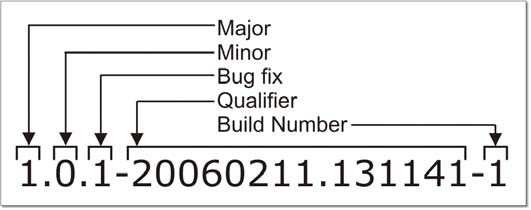
\includegraphics[width=0.65\linewidth]{config-management/major-minor}
  \end{center}
  \caption{Format des Versionsbezeichners (Source: Better Builds mit Maven)}
  \end{figure}
\newslide
Beispiele gültiger Versionsbezeichner:
  \begin{itemize}
  \item 1.0.1-20080211.131141-1
  \item 1.0-alpha
  \item 1.0
  \end{itemize}
  \end{itemize}
  Einige Artefakt-Beispiele:
\begin{center}
\begin{tabular}{lll}
groupId & artifactId & version\\
\hline
junit  & junit & 3.8.1\\
log4j & log4j & 1.2.13\\
mysql & mysql-connector-java & 5.1.5\\
org.springframework & spring & 2.5\\
\end{tabular}
\end{center}
Weitere (aktuell gibt es einige 1000 groupIds) findet man im
offiziellen Maven-Repository:
\href{http://mirrors.ibiblio.org/maven2}{mirrors.ibiblio.org/maven2}

\newslide
Hiermit ist nun die in Abbildung \ref{fig:maven-dirstruct} gezeigte
Verzeichnisstruktur entstanden.
\begin{figure}[H]
  \centering
\ifslides
  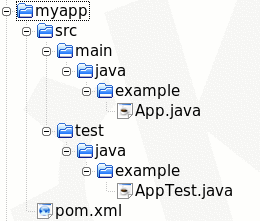
\includegraphics[width=0.4\linewidth]{config-management/maven-dirstruct}
\else
  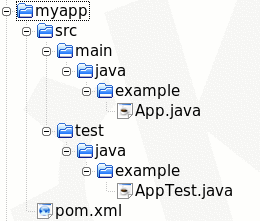
\includegraphics[width=0.4\linewidth]{config-management/maven-dirstruct}
\fi
  \caption{Verzeichnisstruktur eines Maven-Projektes}
  \label{fig:maven-dirstruct}
\end{figure}
\newslide
Mit archetype:generate wird eine Auswahl möglicher Projektvorlagen präsentiert, die mit dem Argument -Dfilter
eingegrenzt werden kann.
%
\newslide
\item \underline{Compilieren und Testen}

Man kann nun auf der Kommandozeile die Aktionen einer bestimmten Projektphase
ausführen. Zum Beispiel:
\begin{lstlisting}
  % mvn test
\end{lstlisting}
Hiermit werden ohne weiteres Zutun die Aktionen aller Phasen bis und
mit der Test-Phase durchgeführt, d.h. es werden die benötigten
Bibliotheken, sofern
nicht vorhanden, heruntergeladen,
die Dateien kompiliert und anschliessend die Unit-Tests
durchgeführt. Dazu werden die Standard-Plugins von Maven verwendet, die
beispielsweise bei Java-Code den Java-1.5-Compiler verwenden.
\newslide
Will man jedoch
 spezifische Compiler-Flags benutzen, muss dies dem
 Plugin \verb+maven-compiler-plugin+ mitgeteilt werden:
\begin{lstlisting}[language=xml,
  morekeywords={plugins,plugin,configuration,artifactId,source,target}]
  <plugins>
    <plugin>
      <artifactId>maven-compiler-plugin</artifactId>
      <configuration>
        <source>1.8</source>
        <target>1.8</target>
      </configuration>
    </plugin>
  </plugins>
\end{lstlisting}
Das Plugins-Element ist Teil des Build-Elementes.
\newslide
\item \underline{Weitere Artefakte verwenden:}

Benötigt man weitere Bibliotheken, dann müssen diese der Dependency-Liste
  hinzugefügt werden. Beispiel:
  \begin{lstlisting}[language=xml,
    morekeywords={dependency,groupId,artifactId,version,scope}]
 <dependency>
   <groupId>log4j</groupId>
   <artifactId>log4j</artifactId>
   <version>1.2.13</version>
   <scope>compile</scope>
 </dependency>
  \end{lstlisting}
Das Maven-Repository kann mit
\href{https://search.maven.org}{search.maven.org}
%\href{http://maven.ozacc.com}{http://maven.ozacc.com} oder
%\href{http://mvnbrowser.com}{mvnbrowser.com}
durchsucht werden.

Maven sorgt dann dafür, dass die entsprechenden Dateien in das lokale
Repository kopiert werden.
%
\newslide
\item \underline{Ausführen}

Das Ausführen gehört nicht eigentlich zu den Kern-Kompetenzen von
Maven. Mit dem Exec-Plugin kann jedoch eine Java-Applikation  wie
folgt ausgeführt werden:
\begin{lstlisting}
mvn exec:java -Dexec.mainClass=example.App
\end{lstlisting}
Allfällige Argumente können mit \verb+-Dexec.args=".."+ übergeben
werden.

Das Exec-Plugin kann auch konfiguriert werden:
\begin{lstlisting}[language=xml,
  morekeywords={plugin,groupId,artifactId,configuration,mainClass}]
<plugin>
  <groupId>org.codehaus.mojo</groupId>
  <artifactId>exec-maven-plugin</artifactId>
  <configuration>
    <mainClass>example.App</mainClass>
  </configuration>
</plugin>
\end{lstlisting}
\newslide
\item \underline{Verpacken:}

Mit dem Parameter package erstellt Maven entsprechend der
Packaging-Property eine Java-Archiv-Datei, die im Verzeichnis
target abgelegt wird. Dabei werden allerdings die abhängigen
Archiv-Dateien nicht mit verpackt. Dies wird vielmehr vom Assembly-Plugin
übernommen:
\begin{lstlisting}[language=xml,
  morekeywords={plugin,artifactId,configuration,descriptorRefs,
  descriptorRef}]
  <plugin>
    <artifactId>maven-assembly-plugin</artifactId>
    <version>3.1.0</version>
    <configuration>
      <descriptorRefs>
        <descriptorRef>jar-with-dependencies</descriptorRef>
      </descriptorRefs>
    </configuration>
  </plugin>
\end{lstlisting}
\newslide
Dieses Plugin ermöglicht es zudem, das Main-Class-Attribut
des Manifests zu definieren:
\begin{lstlisting}[language=xml,
morekeywords={configuration,archive,manifest,mainClass}]
..
    <configuration>
      ..
      <archive>
        <manifest>
          <mainClass>myapp.Main</mainClass>
        </manifest>
      </archive>
      ..
    </configuration>
 ..
\end{lstlisting}
% mvn npackage assembly:single
Die Aktion (das Goal) {\bfseries assembly:single} sorgt
für die eigentliche Erstellung der Archiv-Datei.
Um diese Aktion
 mit der Package-Phase zu verknüpfen, muss das
Execution-Element wie folgt konfiguriert werden:
\begin{lstlisting}[language=xml,
  morekeywords={executions,execution,id,phase,goals,goal}]
  <executions>
    <execution>
      <id>make-assembly</id>
      <phase>package</phase>
      <goals>
        <goal>single</goal>
      </goals>
    </execution>
  </executions>
\end{lstlisting}
Hiermit wird beim Aufruf von Maven mit dem Parameter {\bfseries package} die
Jar-Datei, welche alle Klassen der zu diesem Artefakt abhängigen
Archiv-Dateien enthält.
%
\newslide
\item \underline{Installieren:}

Maven installiert die erstellten Erzeugnisse (Artefakte) in das lokale (private)
Repository und macht sie damit für eigene Maven-Projekte verfügbar:
\begin{lstlisting}
  mvn install
\end{lstlisting}
Bei einer Jar-Datei wird der Pfadname folgt gebildet:
\begin{verbatim}
<groupId>/<artifactId>/<version>/<artifactId>-<version>.jar
\end{verbatim}
Beispiel: org/example/myapp/1.0-SNAPSHOT/myapp-1.0.SNAPSHOT.jar
%
\newslide
\item \underline{Deployment:}

Beim Deployment werden die Artefakte in ein entferntes Repository
kopiert. Dazu werden verschiedene Verfahren unterstützt: File-Copy,
FTP und SCP/SSH.
Zur Konfiguration dient das DistributionManagement-Element:
\begin{lstlisting}[language=xml,
  morekeywords={distributionManagement,repository,id,name,url}]
  <distributionManagement>
    <repository>
      <id>internal.repository</id>
      <name>Internal Repository</name>
      <url>file://${basedir}/target/deploy</url>
    </repository>
  </distributionManagement>
\end{lstlisting}
Bei FTP und SCP/SSH müssen Benutzername/Passwort resp. Public-Key in
der benutzer-spezifischen Settings-Datei \verb+~/.m2/settings.xml+
definiert werden.
\end{enumerate}
% $
\newslide
\subsubsection{Verwendung von Property-Werten}
Properties werden wie bei Ant für
Werte verwendet, die an verschiedenen Stellen referenziert werden:
\begin{lstlisting}[language=xml,
 morekeywords={dependencies,dependency,groupId,artifactId,
   version,scope,properties,junit}]
  <dependencies>
    <dependency>
      ...
      <version>${junit.version}</version>
    </dependency>
  </dependencies>

<properties>
  <junit.version>3.8.1</junit.version>
</properties>
\end{lstlisting}
% $
\newslide
Maven kennt eine Vielzahl implizit definierter Properties:

\begin{tabularx}{\linewidth}{lX}
\verb+project.*+ & Elemente des POM: project.name, project.version\\
\verb+settings.*+ & Benutzerabhängige Maven-Setting-Elemente\\
\verb+env.*+ & Umgebungsvariablen: env.M2\_HOME, env.PATH \\
System Properties & Java-System-Properties: os.name, java.home \ldots\\
\end{tabularx}
\newslide
\subsubsection{Erstellungsvarianten mit Build-Profiles}
Mit Hilfe des Profile-Elementes können unterschiedliche
Erstellungsvarianten konfiguriert werden:
\begin{lstlisting}[language=xml,
  morekeywords={profiles,profile,id,build,plugins,plugin,artifactId,
    configuration,debug,optimize}]
  <profiles>
    <profile>
      <id>production</id>
      <build>
	<plugins>
          <plugin>
            <artifactId>maven-compiler-plugin</artifactId>
	    <configuration>
	      <debug>false</debug>
	      <optimize>true</optimize>
	    </configuration>
	  </plugin>
	</plugins>
      </build>
    </profile>
  </profiles>
\end{lstlisting}
Ein bestimmtes Profile kann mit Angabe des Id-Bezeichners bei der
Ausführung mit der Option -P von Maven festgelegt werden:
\begin{lstlisting}
  mvn -Pproduction compile
\end{lstlisting}
\newslide
\subsubsection{Filtern von Ressourcen}
Für die einfache Anpassung umgebungsabhängiger Konstanten und Texte werden
bei Java-Programmen in der Regel spezielle Ressourcen-Dateien verwendet.
Zum Beispiel können damit der Name und die Version einer Applikation
gesetzt werden:
\begin{lstlisting}[language=java]
  ResourceBundle rb =
     ResourceBundle.getBundle("ApplicationResources");

  String appname = rb.getString("application.name");
  String version = rb.getString("application.version");
  System.out.println("This is " + appname +
                     " (Version " + version + ")");
\end{lstlisting}
\newslide
Legt man im Verzeichnis src/main/resources die Datei
ApplicationResources.properties mit folgendem Inhalt ab
\begin{lstlisting}
# application resources
application.name=${project.name}
application.version=${project.version}
\end{lstlisting}
dann kann Maven dafür sorgen, dass die Property-Werte in der
process-resources-Phase aus der POM-Datei übernommen und eingesetzt
werden.
\newslide
Dazu muss jedoch das
Resource-Element entsprechend konfiguriert werden:
\begin{lstlisting}[language=xml,
morekeywords={build,resources,resource,directory,filtering}]
   <build>
     <resources>
       <resource>
	 <directory>src/main/resources</directory>
	 <filtering>true</filtering>
       </resource>
     </resources>
  </build>
\end{lstlisting}
\newslide
%Die Variable Project enthält die POM-Werte
%
\subsubsection{Test-Durchführung}
Die Durchführung der Unit-Tests ist Bestandteil des
Standard-Build-Prozesses, für welches das Plugin
maven-surefire-plugin zuständig ist:
\begin{lstlisting}
mvn test
\end{lstlisting}
Ohne entsprechende Konfiguration werden alle Tests in den Dateien des
Verzeichnisses src/test und aller Unterverzeichnisse mit folgendem
Muster ausgeführt:
\begin{itemize}
\item \verb+**/Test*.java+
\item \verb+**/*Test.java+
\item \verb+**/*TestCase.java+
\end{itemize}
Dabei können die Testklassen mit TestNG, Junit oder sogar
als normale POJO-Klassen
implementiert werden. Das Plugin berücksichtigt dazu die entsprechende
Dependency-Konfiguration.

Die Ergebnisse werden als
Report-Dateien jeweils in Text- und XML-Format ins Verzeichnis
target/surefire-reports abgelegt und der Build-Prozess wird
abgebrochen, falls ein Unit-Test fehlschlägt.

Dieses Verhalten kann jedoch konfiguriert werden:
\begin{lstlisting}[language=xml,
  morekeywords={plugin,groupId,artifactId,configuration,testFailureIgnore,includes}]
  <plugin>
    <artifactId>maven-surefire-plugin</artifactId>
    <configuration>
      <includes>**/*</includes>
      <testFailureIgnore>false</testFailureIgnore>
    </configuration>
  </plugin>
\end{lstlisting}
%
\newslide
\subsubsection{Reporting}
Mit der Anweisung:
\begin{lstlisting}
% mvn site
\end{lstlisting}
erzeugt Maven eine Projekt-Dokumentation, die im Verzeichnis target/site
abgelegt wird. Die dazu nötigen Informationen werden ebenfalls der
POM-Datei entnommen. Zum Beispiel:
\begin{lstlisting}[language=xml,morekeywords={name,url,description}]
..
  <name>My first Project powered by maven</name>
   <url>http://your.project.url</url>
   <description>Write some brief explanatory text
             about your project.</description>
..
\end{lstlisting}
Das Layout der so erzeugten Dokumentation
kann mit dem File src/site/site.xml angepasst werden.

\newslide
\begin{figure}[H]
\centering
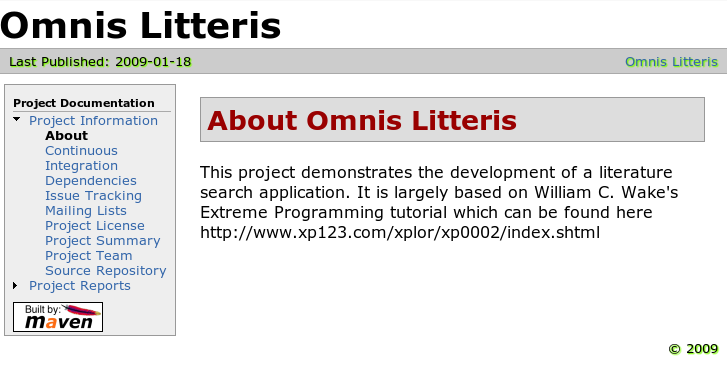
\includegraphics[width=\linewidth]{config-management/mvnsite}
\caption{Eine mit Maven erstellte Projektseite}
\end{figure}
\newslide
Für eine umfassende Dokumentation sorgen zahlreiche Plugins (Beispiele):
\begin{itemize}
\item Change-Log: maven-changelog-plugin
\item Checkstyle: maven-checkstyle-plugin
\item Junit-Report: maven-surefire-report-plugin
\item PMD: maven-pmd-plugin
\item Findbugs: findbugs-maven-plugin
\item JavaDoc: maven-javadoc-plugin
\item Cobertura: cobertura-maven-plugin
\item JXR (Cross-Reference): maven-jxr-plugin
\end{itemize}
\newslide
\begin{lstlisting}[language=xml,
  morekeywords={reporting,plugins,plugin,groupId,artifactId,
    version,configuration}]
  <reporting>
    <plugins>
      <plugin>
	<groupId>org.codehaus.mojo</groupId>
	<artifactId>cobertura-maven-plugin</artifactId>
      </plugin>
      <plugin>
	<artifactId>maven-javadoc-plugin</artifactId>
      </plugin>
      <plugin>
	<artifactId>maven-jxr-plugin</artifactId>
      </plugin>
 ..
    </plugins>
  </reporting>
\end{lstlisting}
\newslide
%\newpage
\newslide
\subsubsection{Eigene Dateien hinzufügen}
Das (lokale) Maven-Repository kann auch mit eigenen Dateien oder solchen,
die man von dritter Seite erhalten hat, ergänzt werden:
\begin{lstlisting}
mvn install:install-file     \
     -Dfile=Sample.jar       \
     -DgroupId=uniquesample  \
     -DartifactId=sample_jar \
     -Dversion=2.1.3b2       \
     -Dpackaging=jar         \
     -DgeneratePom=true
\end{lstlisting}
%
\newslide
\subsubsection{Software Version Control (SCM)}
Mit Hilfe des Plugins \verb+maven-scm-plugin+
bietet Maven auch eine einheitliche Schnittstelle zu
den Source-Code-Management (SCM) Systemen CVS, SVN, GIT (u.a.) an:
\begin{center}
\begin{tabular}{l|l}
Aktion & Beschreibung\\
\hline
 scm:checkin & Änderungen zum SCM-Repository senden\\
 scm:checkout & Arbeitskopie erstellen\\
 scm:add     & Datei hinzufügen\\
 scm:update  & Dateien aktualisieren \\
 scm:status & Status anzeigen\\
 scm:tag    & eine Markierung setzen\\
 \ldots
\end{tabular}
\end{center}
Bei einigen Aktionen müssen Parameter angegeben werden:
\begin{lstlisting}
  % mvn -Dmessage="<checkin comment here>" scm:checkin
\end{lstlisting}
Dazu muss in der POM-Datei das Element scm definiert werden:
\begin{lstlisting}[language=xml,
  morekeywords={scm,connection,developerConnection,url}]
<scm>
  <developerConnection>
    scm:svn:https://somerepository.com/svn_repo/trunk
  </developerConnection>
</scm>
\end{lstlisting}
Bei GIT lautet die URL wie folgt (Beispiel):
\begin{lstlisting}
  scm:git:git://github.com/path_to_repository
\end{lstlisting}
Weitere Infos: \href{http://maven.apache.org/scm/git.html}
                    {maven.apache.org/scm/git.html}
\newslide
\subsubsection{Release-Bildung}
Bei der Release-Bildung überprüft das Release-Plugin die folgenden Punkte:
\begin{itemize}
\item Sind alle lokalen Änderungen mit dem SCM-Repository abgeglichen?
\item Sind alle Integrations-Tests fehlerfrei durchgelaufen?
\item Werden bei den verwendeten Bibliotheken und Plugins
  keine SNAPSHOT-Versionen referenziert?
\end{itemize}
und sorgt dafür, dass die Versionsbezeichner in den POM-Dateien
entsprechend angepasst werden und mit den SCM-Tags korrespondieren:
\begin{lstlisting}
mvn release:prepare -DdryRun=true
\end{lstlisting}
\newslide
Das Plugin verlangt anschliessend die folgenden Angaben:
\begin{itemize}
\item aktueller Versionsbezeichner (Bsp: 1.0)
\item aktueller Releasebezeichner (Bsp: myapp-1.0)
\item neuer Bezeichner der Entwicklungsversion (Bsp: 1.1-SNAPSHOT)
\end{itemize}
und legt die eingebenen Werte in der Datei release.properties
ab. Zusätzlich werden verschiedene POM-Dateien erzeugt, die man
allesamt mit
\begin{lstlisting}
mvn release:clean
\end{lstlisting}
wieder löschen muss, wenn Maven die Aktionen ausführen soll.
\newslide
Nach Eingabe von
\begin{lstlisting}
mvn release:prepare
\end{lstlisting}
% achtung: bei SVN 1.5.2:
%    svn: Commit failed (details follow):
%    svn: File '..' already exists
%
% svn update und ein erneutes mvn:prepare behebt das Problem
%
wird Maven den aktuellen Stand des Projektes in das Tags-Verzeichnis
kopieren, die neue Versionsbezeichnung
in den POM-Dateien einsetzen und mitteilen, dass man nun mit
\begin{lstlisting}
mvn release:perform
\end{lstlisting}
die eigentlichen Release-Dateien bilden und in das lokale (und
Deploy-) Repository
transferieren kann. Damit dieser Schritt klappt, muss das
distributionManagement-Element definiert sein.
% Achtung:
% maven-release-plugin
% configuration tag
%  <plugin>
%        <artifactId>maven-release-plugin</artifactId>
%        <configuration>
%          <tagBase>http://localhost/omnislitteris/tags
%          </tagBase>
%        </configuration>
%      </plugin>
%

Eine verbesserte Unterstützung bietet das Plugin jgitflow:
\begin{lstlisting}[language=xml,morekeywords={plugin,groupId,artifactId,configuration,noDeploy}]
<plugin>
   <groupId>external.atlassian.jgitflow</groupId>
   <artifactId>jgitflow-maven-plugin</artifactId>
   <version>1.0-m5.1</version>
   <configuration>
     <noDeploy>true</noDeploy>
   <configuration>
</plugin>
\end{lstlisting}
Plugin goals:
\begin{itemize}
\item \structure{jgitflow:release-start} create and push a release branch
\item \structure{jgitflow:release-finish} build, tag and merge the release branch
into master and develop branches
\end{itemize}
\newslide
\subsubsection{Exercise}
\begin{enumerate}
\item Konvertieren Sie das Projekt Histogram in ein Maven-Projekt
(artifactId: histogram, groupId=demo) und
erstellen Sie die ausführbare Archiv-Datei mit allen benötigten Klassen.
Wie lautet der Dateiname der Archiv-Datei, und wie kann man ihn
konfigurieren?

%Hinweis: Bis und mit Version 1.0.12
%wird von jfreechart  die Library gnujaxp benötigt, welche
%nicht im offiziellen Maven-Repository abgelegt ist. Sie müssen
%in diesem Fall Ihre
%POM-Datei mit dem folgenden Repositories-Element ergänzen:
%\begin{lstlisting}[language=xml,
%   morekeywords={repositories,repository,id,name,url}]
%  <repositories>
%    <repository>
%      <id>maven-repository.atlassian.com</id>
%      <name>Atlassian Maven Repository</name>
%      <url>http://maven.atlassian.com/repository/public</url>
%    </repository>
%  </repositories>
%\end{lstlisting}
\end{enumerate}
%
\subsubsection{Software and further Informations}
\begin{itemize}
\item Maven: \href{http://maven.apache.org/}{maven.apache.org/}
\item Maven, The Definitive Guide
%(Tim O'Brien, John Casey, Brian Fox, Bruce Snyder, Jason Van Zyl)

\href{http://www.sonatype.com/book/reference/public-book.html}
{www.sonatype.com/book/reference/public-book.html}

\item Eclipse und Maven:
  \href{http://www.eclipse.org/m2e/}{www.eclipse.org/m2e/}
%\item An introduction to Maven 2
%
%\href{http://www.javaworld.com/javaworld/jw-12-2005/jw-1205-maven.html}
%   {www.javaworld.com/javaworld/jw-12-2005/jw-1205-maven.html}
%
%\item Building Web Applications with Maven
%
%   \href{http://today.java.net/pub/a/today/2007/03/01/building-web-applications-with-maven-2.html}
%      {today.java.net/pub/a/today/2007/03/01/building-web-applications-with-maven-2.html}
%
%\item Maven 2.0: Compile, Test, Run, Deploy, and More
%
%\href{http://www.onjava.com/pub/a/onjava/2006/03/29/maven-2-0.html}
%{www.onjava.com/pub/a/onjava/2006/03/29/maven-2-0.html}
%
%\item Get the most out of Maven 2 site generation:
%
%\href{http://www.javaworld.com/javaworld/jw-02-2006/jw-0227-maven.html}
%  {www.javaworld.com/javaworld/jw-02-2006/jw-0227-maven.html}
%
%\item Introduction to Apache Maven 2
%
%\href{http://www-128.ibm.com/developerworks/edu/j-dw-java-mavenv2.html}
%   {www-128.ibm.com/developerworks/edu/j-dw-java-mavenv2.html}
%
%\item Tutorial:Hibernate, Spring, HSQL, Eclipse \& Maven
%
%\href{http://www.lulu.com/content/1087191}{www.lulu.com/content/1087191}
%
%\item Netbeans Wiki: Maven best practices
%
%\href{http://wiki.netbeans.org/MavenBestPractices}
%  {wiki.netbeans.org/MavenBestPractices}
%
%\item Working with Maven in Netbeans
%
%\href{http://today.java.net/article/2009/10/14/working-maven-netbeans-671}
%  {today.java.net/article/2009/10/14/working-maven-netbeans-671}
\end{itemize}

\newpage
%\section*{Konfigurationsmanagement}
\section{Bug/Issue Tracking}
\subsection{Bugzilla}
Bugzilla ist ein von Terry Weissmann ursprünglich in TCL jetzt in Perl
geschriebenes
Problembehandlungssystem, welches im Open-Source-Umfeld einen
Defacto-Standard darstellt.
\begin{center}

\includegraphics[width=0.18\linewidth]{config-management/buggie}\hfill
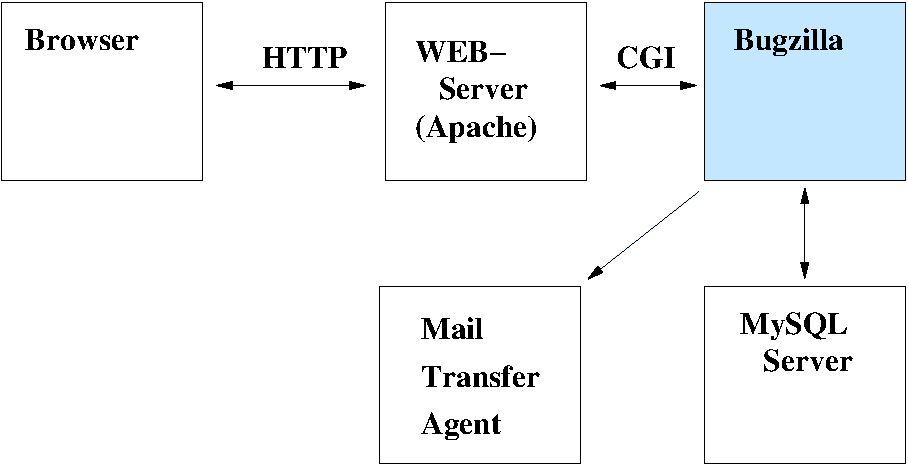
\includegraphics[width=0.56\linewidth]{config-management/xfig/bugzilla}
\end{center}
Bugzilla bietet:

\begin{minipage}{0.48\linewidth}
\begin{itemize}
\item vielfältige Suchmöglichkeiten:
  \begin{itemize}
  \item Welche Probleme sind bekannt, werden bearbeitet, sind behoben?
  \item Welche Releases sind davon betroffen?
  \item Wer ist für das Problem zuständig?
  \item Wie lautet die Problemlösung?
  \end{itemize}
\end{itemize}
\end{minipage}\hfill
\begin{minipage}{0.48\linewidth}
\begin{itemize}
\item vollständige Dokumentationen der Modifikationen (Reports, Grafiken),
\item konfigurierbare Benachrichtigungen bei \"Anderungen,
\item unterschiedliche Schnittstellen: E-Mail, Web, XML, Konsole.
\end{itemize}
\end{minipage}
\begin{figure}[H]
\centering
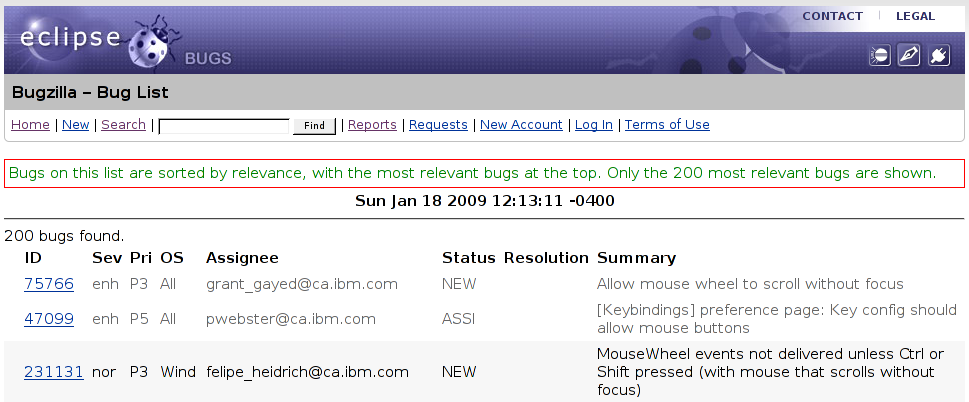
\includegraphics[width=0.85\linewidth]{config-management/bugzilla-buglist1}
\caption{Anzeige der Bug-Liste}
\end{figure}
%---------------------------------------------------------------
\newpage
\ifslides
\begin{center}
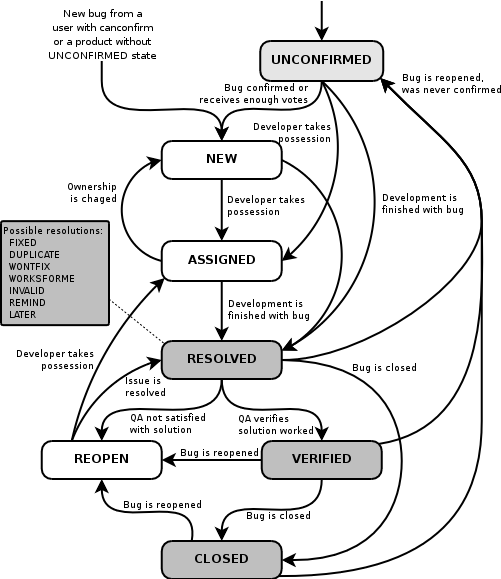
\includegraphics[width= 0.6\linewidth]{config-management/bzLifecycle}
\end{center}
\else
\subsubsection{Zustandsmodell}
\begin{figure}[H]
\caption{Lifecycle of a Bug}
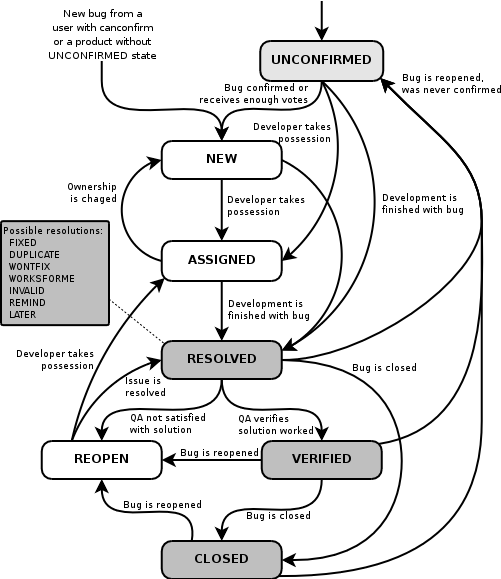
\includegraphics[width= \linewidth]{config-management/bzLifecycle}
\end{figure}
\fi
\newpage
\subsubsection{Aufbau einer Problemmeldung:}
\ifslides
\else
%Aufbau einer Problemmeldung:\\[2ex]
\fi
\ifslides
{\small
\fi
\begin{tabular}{lp{9.5cm}}
\hline
Product und Component & Ein Produkt kann aus mehreren Komponenten bestehen\\
Status & Zustand der Problemmeldung: UNCONFIRMED, NEW, ASSIGNED, REOPENED,
RESOLVED, VERIFIED, CLOSED\\
Resolution & Behebung: FIXED, INVALID, WONTFIX, LATER, REMIND, DUPLICATE,
WORKSFORME, MOVED\\
Assigned to & die für die Behebung zuständige Person\\
URL & ein mit diesem Problem verknüpfter URL (falls vorhanden)\\
Summary & Zusammenfassung\\
Whiteboard & Beschreibung des Problems\\
Keywords & wichtige Schlüsselbezeichner\\
\ifslides
\end{tabular}
}
\newpage
{\small
\begin{tabular}{lp{9.5cm}}
\fi
Platform und OS & Rechnertyp und Betriebssystem\\
Version & Versionsnummer (Release) des betreffenden Produktes/der Komponente\\
Priority & zugewiesene Priorität: P1 - P5\\
Severity & Auswirkung: blocker, critical, major, normal, minor, trivial,
enhancement\\
Target & voraussichtlicher Release, mit dem das Problem behoben sein wird\\
Reporter & Person, die das Problem gemeldet hat\\
CC & Personen, die bei \"Anderungen des Problemzustandes benachrichtigt
werden\\
Attachments & beiliegende Dateien\\
Dependencies & Abhängigkeiten\\
%%Votes & \\
Comments & Kommentare\\
\hline
\end{tabular}
\ifslides
}
\newpage
\fi
\subsubsection{Suchen von Bugs mit Bugzilla}
\ifslides
\begin{center}
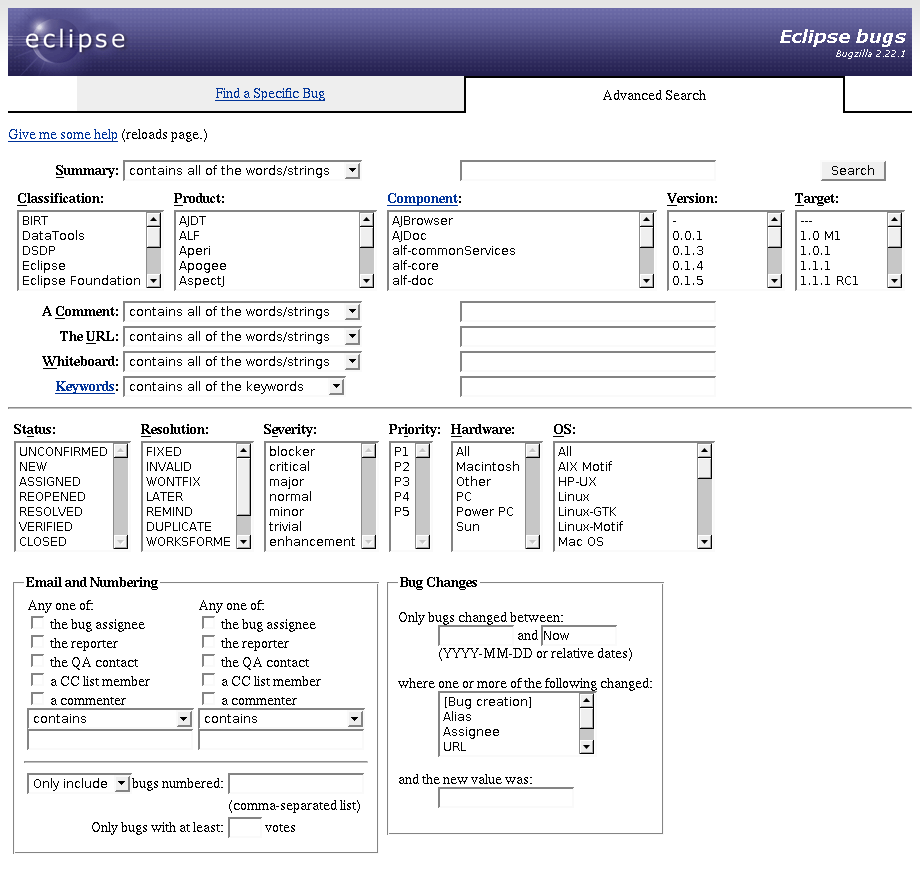
\includegraphics[width=0.6\linewidth]{config-management/bugzilla-search}
\end{center}
\else
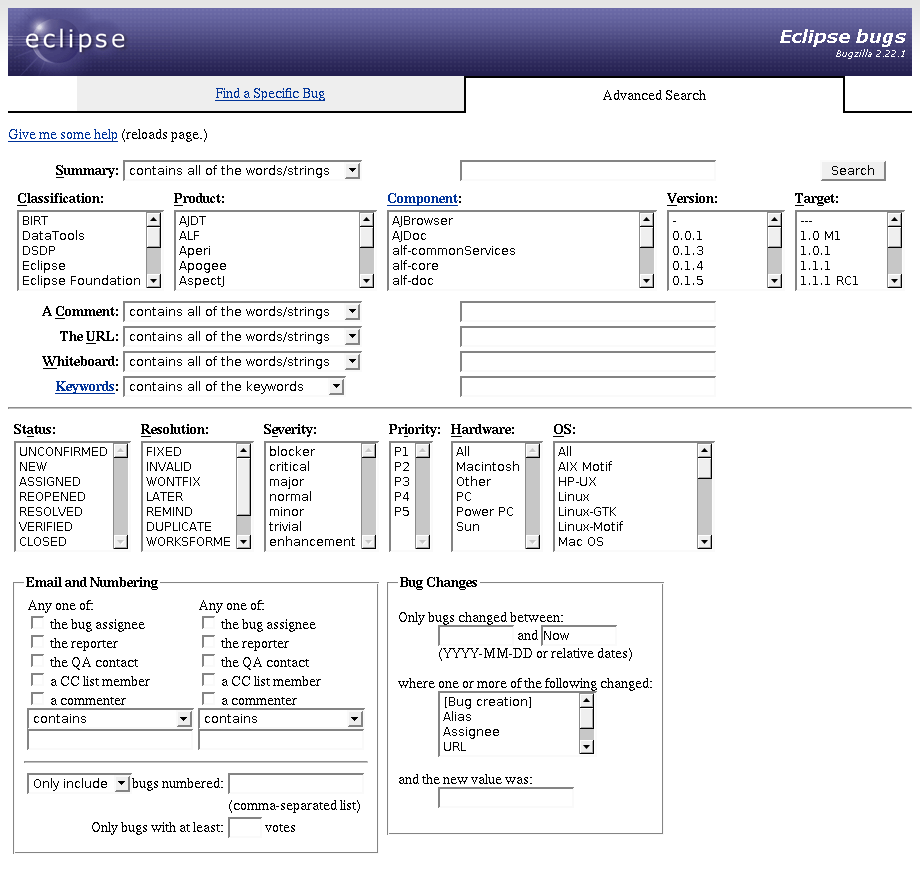
\includegraphics[width=\linewidth]{config-management/bugzilla-search}
\fi
%\newpage
%\subsubsection{Installation und Konfiguration von Bugzilla}
%Bugzilla kann grundsätzlich auf Mac, Windows und Unix/Linux-Systemen betrieben
%werden. Am einfachsten ist die Installation auf Linux (Details siehe
%Dokumentation):
%\begin{enumerate}
%\item Man installiert, falls nicht bereits vorhanden, Perl, Apache und MySQL.
%\item Man lädt eine aktuelle Bugzilla-Version herunter (2.22) und entpackt
%  sie in ein lokales (Web-) Verzeichnis
%  (z.B. /srv/www/htdocs/bugzilla-2.22). Der Web-Server-User (\verb+wwwrun+)
%  soll Schreibrechte in diesem Verzeichnis haben.
%\item Man installiert allenfalls zusätzlich benötigte
%  Perl-Module:
%  \begin{lstlisting}[language=ksh]
%    checksetup.pl --check-modules
%    perl -MCPAN -e 'install "<modulename>"'
%  \end{lstlisting}
%\item Man installiert einen MTA (sendmail, postfix, exim \ldots), der bei
%  Systemstart gestartet wird.
%\item Man konfiguriert Bugzilla:
%  \begin{enumerate}
%  \item Das Benutzerpasswort für den Datenbank-Benutzer \verb+bugs+.
%\ifslides
%\else
%  (Datei:\verb+localconfig+).
%\fi
%\item Verschiedene MySQL-Parameter: die maximal zulässige Grösse der
%  Attachments,
%  die minimale Wortlänge für die Index-Suche, die maximale Tabellengrösse.
%\item Man legt den Datenbank-Benutzer \verb+bugs+ an und gibt ihm die nötigen
%  Berechtigungen.
%\item Man führt das Skript \verb+checksetup.pl+ aus, welches die Tabellen
%  erzeugt und nach Bedarf weitere Administratoren anlegt.
%  \end{enumerate}
%\item Man konfiguriert den Web-Server, so dass CGI-Skripte im
%  Bugzilla-Verzeichnis ausgeführt werden können (File \verb+httpd.conf+).
%\end{enumerate}
%Bugzilla bietet eine Vielzahl von Konfigurationsmöglichkeiten. Zum Beispiel
%können auf der Basis von Benutzergruppen die Rechte für die Anzeige, das
%Erfassen und Ändern von Einträgen produkt-spezifisch zugeteilt werden.

%\newpage
%\input{mantis}
%\newpage
% http://gushieblog.blogspot.com/2006/11/trac.html
% http://trac-hacks.org/wiki/GitPlugin
%
\subsection{Trac}
\begin{minipage}{0.55\linewidth}
Trac ist ein erweiterbares Bug-Tracking-Werkzeug mit einer einfachen
Projekt-Management-Funktionalität.
Zusätzlich bietet das von der Firma Edgewood ebenfalls in
Open-Source-Lizenz entwickelte Tool
ein Wiki-System sowie eine Schnittstelle zu verschiedenen Versionsverwaltung-Systemen
(ua. Subversion und Git). Trac basiert auf der Scriptsprache Python und kann
an unterschiedliche Datenbanken angepasst werden.
\end{minipage}
\hfill
\begin{minipage}{0.4\linewidth}

\includegraphics[width=\linewidth]{config-management/trac_diagram}
\end{minipage}
%
\ifslides
\begin{center}
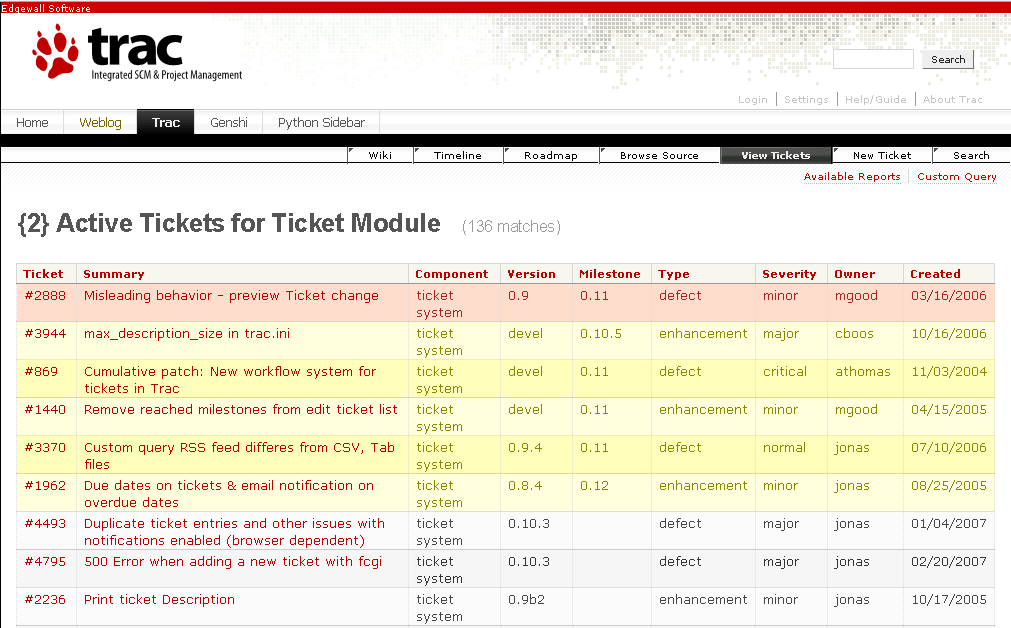
\includegraphics[width=\linewidth]{config-management/trac-ticketlist}
\end{center}
\else
\begin{figure}[H]
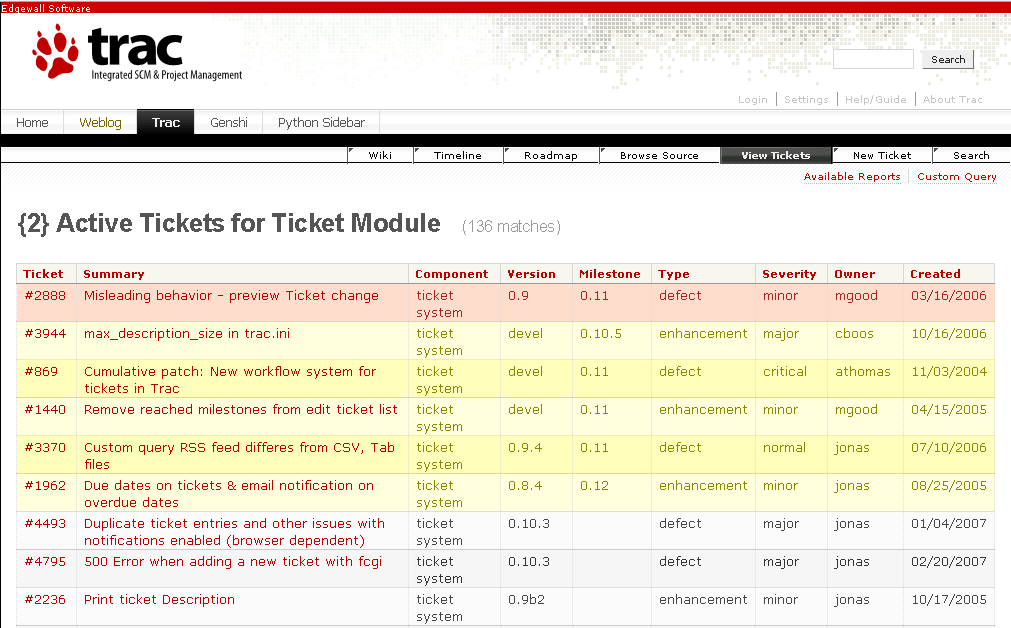
\includegraphics[width=\linewidth]{config-management/trac-ticketlist}
\caption{Anzeige der Ticket-Liste bei Trac}
\end{figure}
\fi
\ifslides
\begin{figure}[H]
\begin{center}
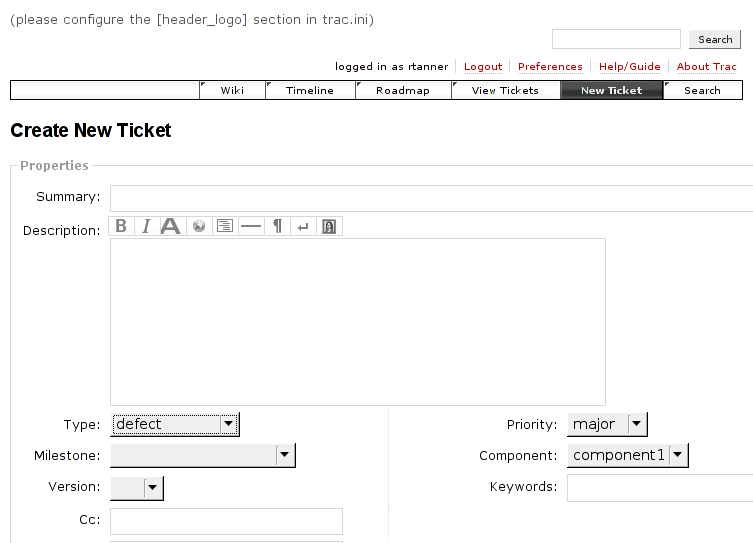
\includegraphics[width=0.7\linewidth]{config-management/trac-newticket}
\caption{Erfassen eines Tickets bei Trac}
\end{center}
\end{figure}
\else
\begin{figure}[H]
\begin{center}
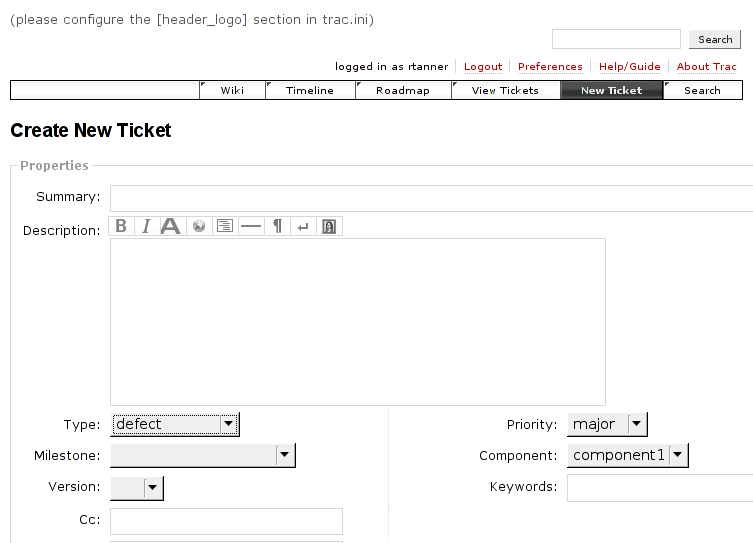
\includegraphics[width=0.8\linewidth]{config-management/trac-newticket}
\caption{Erfassen eines Tickets bei Trac}
\end{center}
\end{figure}
\fi
%
\ifslides
\begin{figure}[H]
\begin{center}
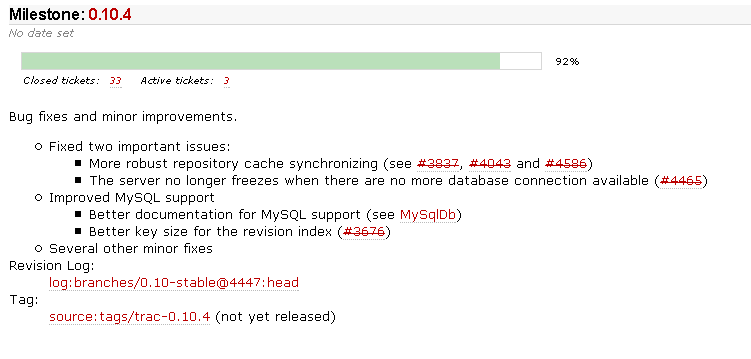
\includegraphics[width=\linewidth]{config-management/trac-roadmap}
\caption{Roadmap bei Trac}
\end{center}
\end{figure}
\else
\begin{figure}[H]
\begin{center}
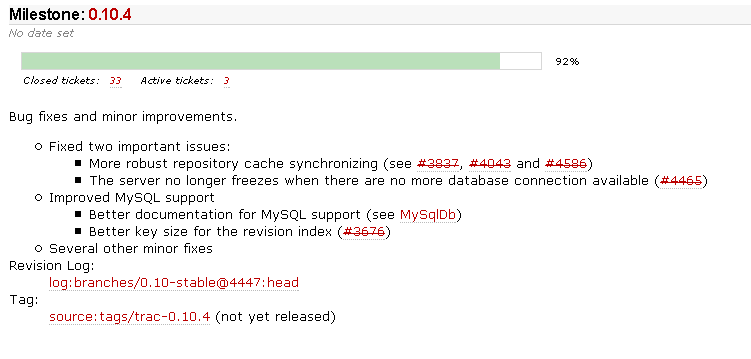
\includegraphics[width=0.8\linewidth]{config-management/trac-roadmap}
\caption{Roadmap bei Trac}
\end{center}
\end{figure}
\fi
\subsubsection{Workflow}
Beim Arbeiten mit Trac muss einer konfigurierten Abfolge von Schritten,
einem sogenannten Workflow, der vom Zustand
des Tickets gesteuert wird, gefolgt werden. Die Workflow-Regeln können im
Konfigurations-File trac.ini festgelegt werden. Bei der
Installation von Trac wird der in Abbildung \ref{fig:trac-workflow}
dargestellte Workflow eingestellt.
\begin{figure}[H]
  \centering
  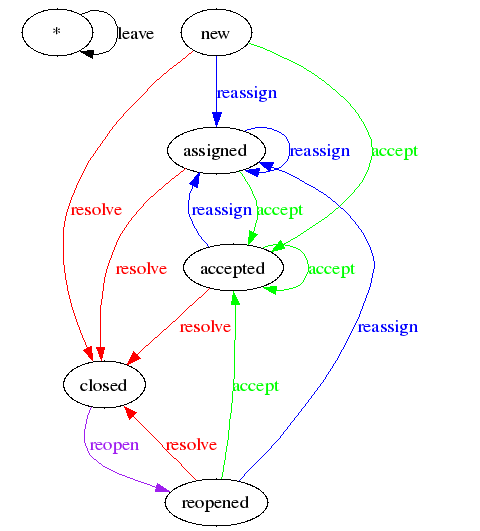
\includegraphics[width=0.5\linewidth]{config-management/trac-workflow}
  \caption{Default-Workflow}
  \label{fig:trac-workflow}
\end{figure}
%
\paragraph{\underline{1. Erfassen eines Tickets}}
Ein angemeldeter Benutzer mit der zugeteilten Berechtigung
\verb+TICKET_CREATE+ kann ein neues Ticket erfassen.
Ein Ticket kann eine Fehlermeldung, ein
  Änderungsvorschlag, eine Idee für eine Erweiterung sein.
  Es müssen dabei die folgenden Informationen
  eingeben werden:
  \begin{description}
    \item [Summary] eine Kurzbeschreibung des Inhalts
    \item [Description] die ausführliche Beschreibung
    \item[Type] der Typ des Tickets:
      \begin{itemize}
      \item defect: ein Bug, eine Störung, etwas was nicht so
        funktioniert, wie es
        erwartet wird oder dokumentiert ist,
      \item enhancement: eine Erweiterung, Verbesserung des
        bestehenden Systems,
      \item Task: ein Auftrag, der erledigt werden muss/sollte
      \end{itemize}
      Die Liste kann vom Administrator geändert und ergänzt werden.
\newslide
      \item [Priority:] die Auswirkung resp. Dringlichkeit
        \begin{center}
        \begin{tabular}{llll}
          Priority & Weiterarbeit & Verbesserung & Behebung/Umsetzung\\
          \hline
         {\bfseries blocker} &  nicht möglich & unverzichtbar & unverzüglich \\
         {\bfseries critical} & erheblich eingeschränkt & bedeutend & möglichst bald\\
       {\bfseries major} & eingeschränkt & wichtig & innerhalb kurzer Zeit\\
        {\bfseries minor} & leicht eingeschränkt & geringfügig & bald \\
        {\bfseries trivial} & marginal eingeschränkt & kosmetisch & offen \\
      \end{tabular}
    \end{center}
\newslide
  \item[Milestone] der Release, bei welchem das Problem behoben sein
    sollte,
  \item[Component] die betroffene Komponente (Teilsystem),
  \item[Version] die betroffene Version des verwendeten Systems (nur
    bei defects),
  \item[CC] E-Mail-Adressen und/oder Benutzer, die bei Änderungen
    benachrichtigt werden sollen,
   \item[Estimated Number of Hours] der geschätzte Aufwand in Stunden,
   \item[Add hours to ticket] der neu geleistete Aufwand in Stunden,
   \item[Assign to] die für die Behebung zuständige Person,
   \item[I have files to attach] wenn Dateien (Screenshots,
     Log-Dateien, Patches\ldots) hinzugefügt werden sollen.
  \end{description}
%
\newslide
\paragraph{\underline{2. Bearbeiten eines Tickets}}
Nachdem ein Ticket erfasst ist, kann es von jedem Benutzer mit der zugeteilten
Berechtigung \verb+TICKET_MODIFY+ modifiziert werden. Alle Änderungen
werden mit Datum und Benutzername aufgezeichnet.
%und können mit den
%Menupunkten ''View Tickets'' oder ''Timeline'' angezeigt werden.

Tickets können auf unterschiedliche Art gesucht und angezeigt werden:
\begin{itemize}
\item Search: Eingabe eines Such-Textes
\item View Tickets: Ausgabe einer sortierten Ticket-Liste nach unterschiedlichen
  Filter- und Gruppierkriterieren:
  \begin{itemize}
  \item active: alle Tickets, die noch nicht abgeschlossen sind,
  \item active by version: dito, gruppiert nach Version,
  \item active tickets by milestone: dito, gruppiert nach Milestone,
  \item accepted by owner: alle Tickets, die akzeptiert aber noch
    nicht abgeschlossen sind, gruppiert nach Besitzer,
  \item all by milestone: alle Tickets gruppiert nach Milestone
  \item my tickets: alle Tickets, die dem Benutzer zugewiesen sind
  \end{itemize}
\end{itemize}
\newslide
Wenn ein Ticket erfasst worden ist, erhält es den Zustand ''New''. Es
muss innerhalb einer festzulegenden Periode geprüft, fehlende oder
inkorrekte Einträge müssen korrigiert oder ergänzt und einem
Bearbeiter zugewiesen, resp. von einem Bearbeiter akzeptiert
werden. Insbesondere müssen vor einer Zuweisung die folgenden Werte
korrekt gesetzt werden:
\begin{itemize}
  \item Milestone
  \item Version (nur bei einem defect)
\end{itemize}
Ein zugewiesenes Ticket muss von einem Bearbeiter akzeptiert
werden. Er setzt dabei den geschätzten Aufwand im Textfeld ''estimated
number of hours''.
%
\newslide
\paragraph{\underline{3. Abschliessen eines Tickets}}
Das Ticket wird mit ''resolve as'' und der Angabe des geleisteten Aufwands
geschlossen. Dabei muss eines der folgenden
Attribute gewählt werden:
\begin{description}
\item[fixed] das Problem ist behoben resp. die Verbesserung ist
  implementiert, getestet und eingecheckt.
\item[invalid] das Ticket ist ungültig, weil es entweder einen
  Sachverhalt beschreibt, der beabsichtigt ist, oder weil das Problem
  ein anderes System betrifft.
\item[wontfix] das beschriebene Problem kann aus technischen oder
  ökonomischen Gründen nicht behoben werden.
\item[duplicate] das Problem ist bereits von einem anderen Ticket beschrieben.
\item[worksforme] das Problem kann nicht reproduziert werden.
\end{description}
Der jeweilige Entscheid muss im Textfeld ''Add/Change'' begründet werden.

Ein bereits geschlossenes Ticket kann mit ''reopen' wieder geöffnet werden.
%
\newpage
\subsection{Gitlab: Issues}
\ifslides
\begin{picture}(0,0)
\put(250,22){
  
\includegraphics[width=4cm]{config-management/gitlab-logo}
}
\end{picture}
\else
\begin{picture}(0,0)
\put(280,17){
  
\includegraphics[width=3.7cm]{config-management/gitlab-logo}
}
\end{picture}
\fi
The GitLab issue tracker is an advanced tool for collaboratively
developing ideas, solving problems, and planning work.
\begin{figure}[H]
  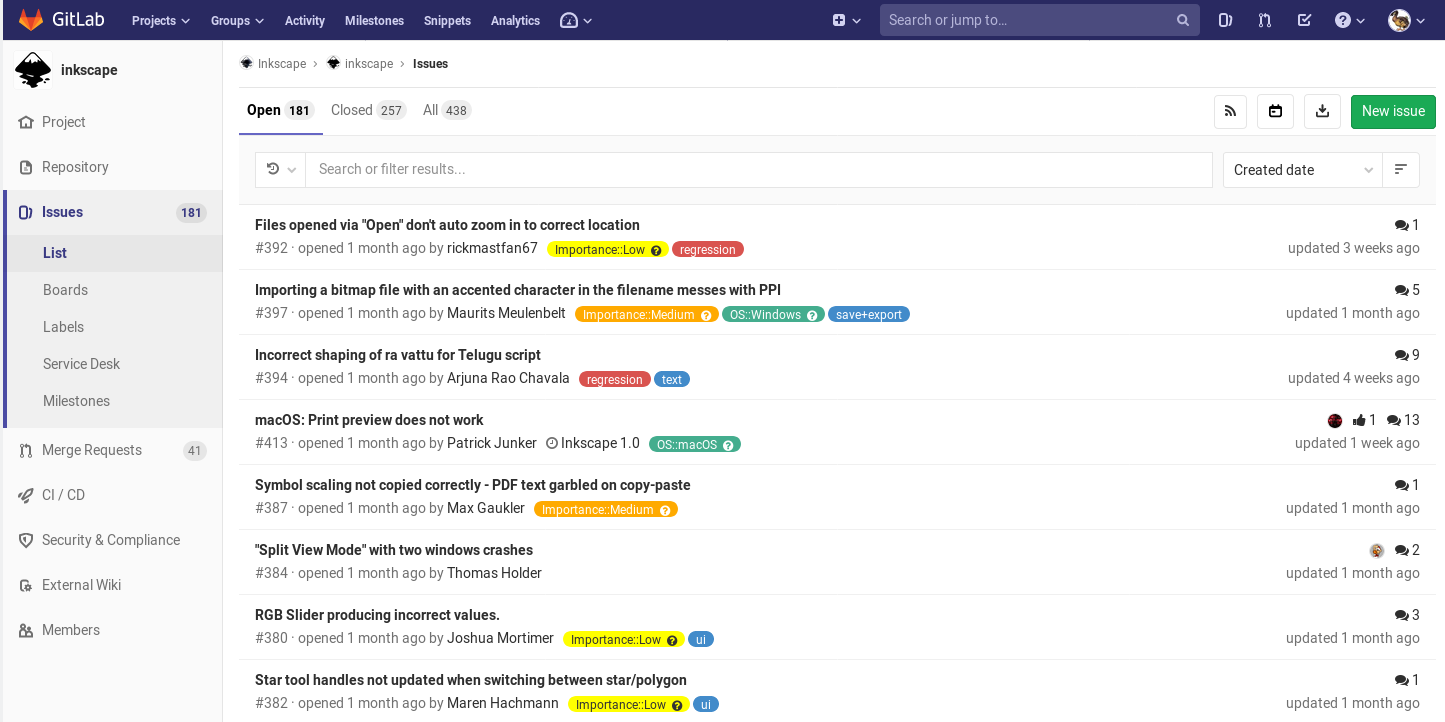
\includegraphics[width=\linewidth]{config-management/gitlab-issues}
  \caption{Gitlab Issue Example}
\end{figure}
\begin{figure}[H]
  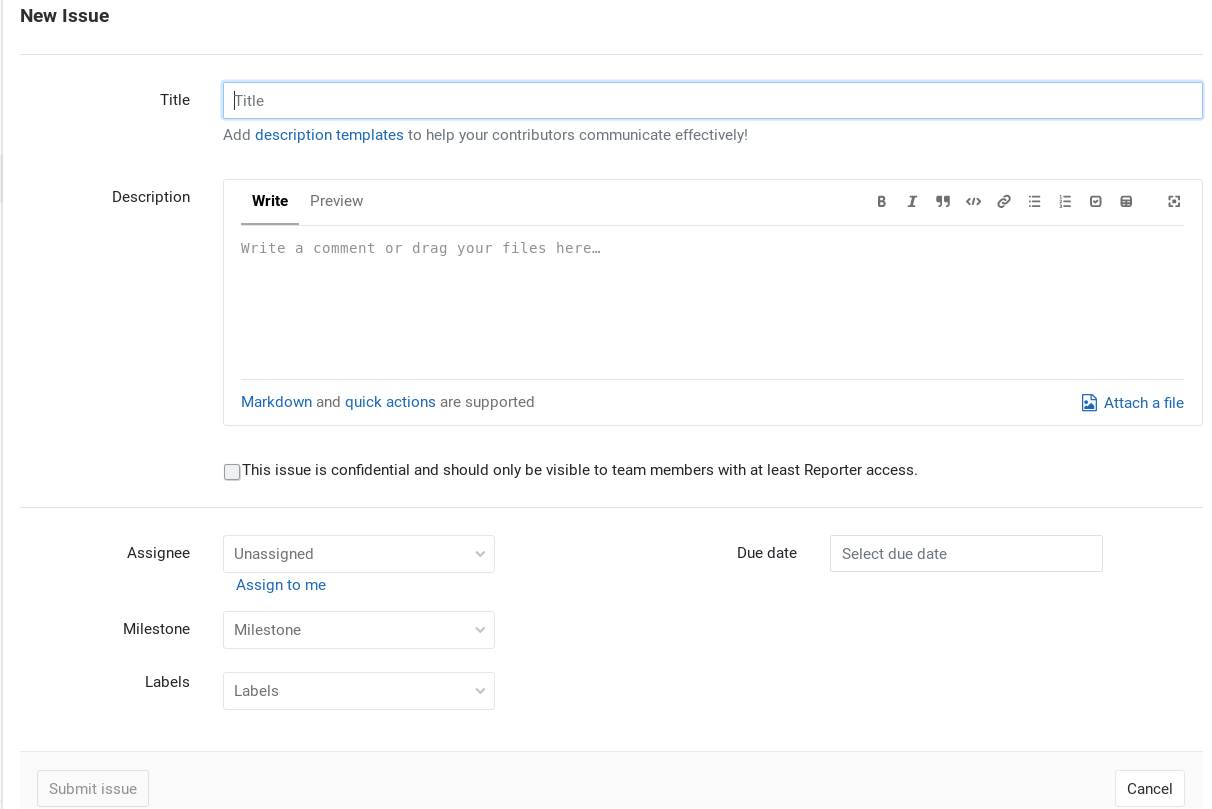
\includegraphics[width=\linewidth]{config-management/gitlab-new-issue}
  \caption{Gitlab New Issue}
\end{figure}
Concepts:
\begin{description}
\item[Labels]: categorize issues or merge requests using descriptive titles like bug, feature request, or docs
\item[Issue Boards]: groups issues in lists that correspond to their assigned labels,
  visualizing issues designed as cards throughout those lists.
\item[Milestones]: group issues and merge requests with an optional start date and an optional due date.
\end{description}

\newpage
\subsection{JIRA}
\ifslides
\begin{picture}(0,0)
\put(270,22){

\includegraphics[width=2.5cm]{config-management/jira-logo}
}
\else
\begin{picture}(0,0)
\put(300,22){

\includegraphics[width=2.5cm]{config-management/jira-logo}
}
\fi
\end{picture}
JIRA ist ein Problemverwaltungsystem, oder vielleicht zutreffender,
ein kommerzielles, populäres, umfassendes, konfigurierbares Pendenzen- und
Projektverwaltungssystem
(Issue Tracking and Project Management) auf Java-EE-Basis.
%welches für Non-Profit-Organisationen und Open-Source-Projekte
%kostenfrei eingesetzt werden kann.
\ifslides
\begin{figure}[H]
\begin{center}
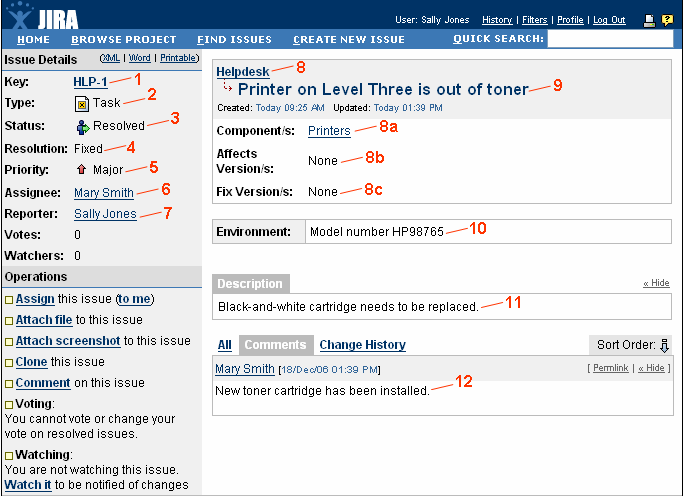
\includegraphics[width=0.9\linewidth]{config-management/jira-issue-overview}
\end{center}
\caption{Anzeigen einer Pendenz bei JIRA}
\end{figure}
\else
\begin{figure}[H]
\begin{center}
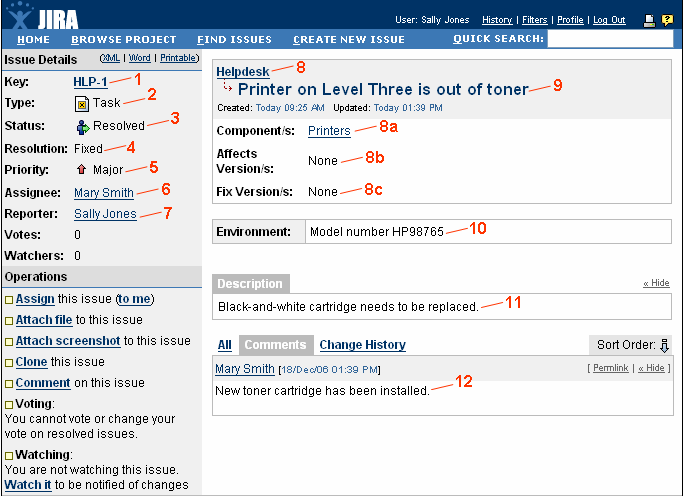
\includegraphics[width=\linewidth]{config-management/jira-issue-overview}
\end{center}
\caption{Anzeigen einer Pendenz bei JIRA}
\end{figure}
\fi
%
\begin{enumerate}
\item {\bfseries Key}: ein eindeutiger Kennzeichner.
\item {\bfseries Type}: Bug, Improvement, New feature, Task, Custom issue
\item {\bfseries Status}: der Zustand, den die Pendenz gegenwärtig einnimmt:
   Open, In Progress, Resolved, Reopened, Closed.
\item {\bfseries Resolution}: ob und wie die Pendenz erledigt ist:
  Fixed, Won't Fix, Duplicate, Incomplete, Cannot Reproduce.
\item {\bfseries Priority}: die Wichtigkeit in Bezug zu anderen Pendenzen:
   Blocker, Critical, Major, Minor, Trivial.
\item {\bfseries Assignee}: die Person, welcher die Pendenz zugewiesen ist.
\item {\bfseries Reporter}: die Person, die die Pendenz erfasst hat.
\newslide
\item {\bfseries Project}:  das zugeordnete Projekt
\begin{enumerate}
  \item Component(s): die betroffenen Projekt-Komponenten
  \item Affects Version(s): die betroffenen Versionen
  \item Fix Version(s)*: die Projekt-Versionen, bei welchen das
      Problem behoben ist (oder sein wird)
  \end{enumerate}
\item {\bfseries Summary}: eine Kurzbeschreibung
\item {\bfseries Environment}*
  die betroffene Hardware oder Software-Umgebung
\item {\bfseries Description} die detaillierte, (nachvollziehbare!) Beschreibung
\item {\bfseries Comments}: allfällige Kommentare der Bearbeiter
  \end{enumerate}
%
\begin{figure}[H]
\begin{center}
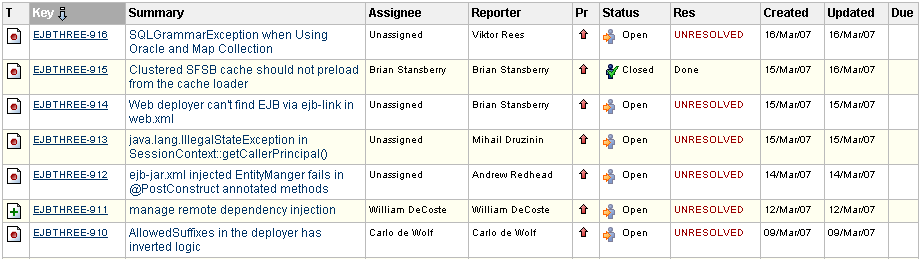
\includegraphics[width=\linewidth]{config-management/jira-issue-list}
\end{center}
\caption{Eine Pendenzenliste bei JIRA}
\end{figure}
%
\begin{figure}[H]
\begin{center}
\ifslides
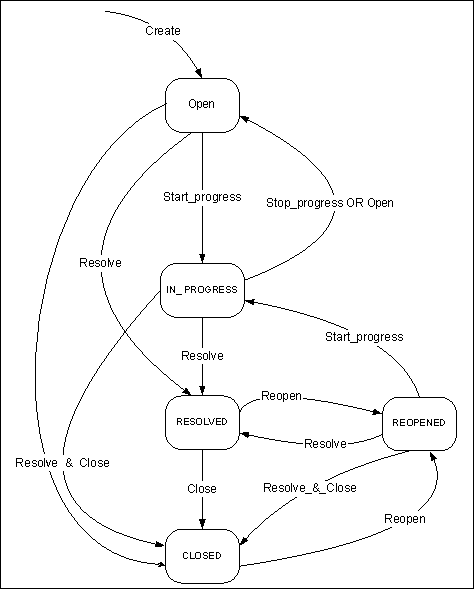
\includegraphics[width=0.4\linewidth]{config-management/jira-workflow-statediagram}
\else
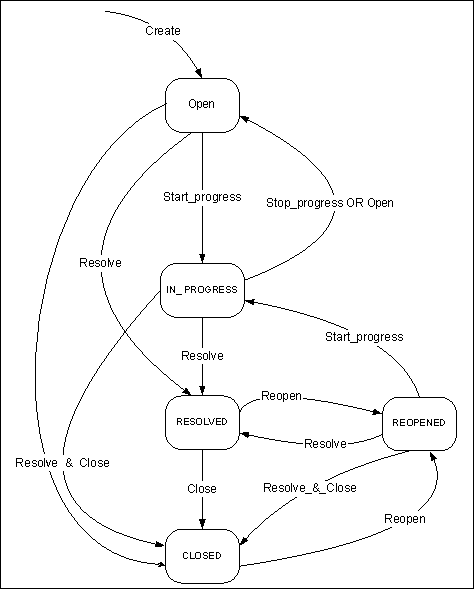
\includegraphics[width=0.6\linewidth]{config-management/jira-workflow-statediagram}
\fi
\end{center}
\caption{Default-Workflow bei JIRA}
\end{figure}
%

%
\newpage
\section{Exercises}
\begin{enumerate}
\item Untersuchen und vergleichen Sie die Charakteristiken
  verschiedener Projekte, die Bugzilla, Mantis, JIRA oder
  Trac einsetzen. Welchen betrieblichen Nutzen haben
  diese Bug-Tracking-Systeme?
  Welche Reporting-Möglichkeiten gibt es und welche
  geschäftsrelevanten Schlüsse lassen sich daraus ziehen?
\item Führen Sie mit Trac oder Gitlab für das Histogram-Projekt
die folgenden Schritte durch:
\begin{enumerate}
\item Erstellen Sie die Meilensteine ``rel-0.0'', ``rel-0.1'' und ``rel-0.2''
\item Erstellen Sie die Tickets/Issues
  \begin{itemize}
  \item Einrichten des Projektes,
  \item Erstellen einer ausführbaren JAR-Datei mit Ant
  \item Erstellen einer ausführbaren JAR-Datei mit Maven
  \end{itemize}
 und weisen Sie die Tickets jeweils einem Meilenstein zu.
\end{enumerate}
\end{enumerate}
%{\bfseries Bewertung:} Vollständigkeit, Korrektheit, Nachvollziehbarkeit
%
\newslide
\subsection{Software and further Informationa}
\begin{itemize}
\item Bugzilla: \href{https://www.bugzilla.org}{www.bugzilla.org}
%\item Bugzilla Test Server: \href{http://landfill.bugzilla.org}
%                                 {landfill.bugzilla.org}
\item Trac: Integrated SCM and Project Management
% an enhanced wiki and issue tracking system for software
%  development projects.
  \href{https://www.edgewall.org/trac}{www.edgewall.org/trac}
  \item Gitlab: \href{https://docs.gitlab.com/ee/README.html}{docs.gitlab.com/ee/README.html}
\item Mantis BT: \href{https://www.mantisbt.org}
  {www.mantisbt.org}
\item Redmine \href{https://www.redmine.org}{www.redmine.org}
\item JIRA: \href{https://www.atlassian.com/software/jira}
  {www.atlassian.com/software/jira}
\end{itemize}
\newpage
